\documentclass[a4paper,onecolumn,oneside,12pt,extrafontsizes]{memoir}
% W celu przygotowania wydruku do archiwum należy przesłonić komendę powyższą
% dwoma poniższymi komendami:
%\documentclass[a4paper,onecolumn,twoside,10pt]{memoir} 
%\renewcommand{\normalsize}{\fontsize{8pt}{10pt}\selectfont}

%\usepackage[cp1250]{inputenc} % jeśli kodowanie edytowanych plików to cp1250 
\usepackage[utf8]{inputenc} % jeśli kodowanie edytowanych plików to UTF8
\usepackage[T1]{fontenc}
\usepackage[polish]{babel}
%\DisemulatePackage{setspace}
\usepackage{setspace}
\usepackage{tabularx}
\usepackage{float}
\usepackage{color,calc}
\usepackage{ebgaramond}
\usepackage{tgtermes}   
\renewcommand*\ttdefault{txtt}
% \usepackage{listings} % pakiet do prezentacji kodu. 
\usepackage{caption}
\usepackage{listings, xcolor}
\lstset{literate=%-
{ą}{{\k{a}}}1 {ć}{{\'c}}1 {ę}{{\k{e}}}1 {ł}{{\l{}}}1 {ń}{{\'n}}1 {ó}{{\'o}}1 {ś}{{\'s}}1 {ż}{{\.z}}1 {ź}{{\'z}}1 {Ą}{{\k{A}}}1 {Ć}{{\'C}}1 {Ę}{{\k{E}}}1 {Ł}{{\L{}}}1 {Ń}{{\'N}}1 {Ó}{{\'O}}1 {Ś}{{\'S}}1 {Ż}{{\.Z}}1 {Ź}{{\'Z}}1 }%{\ \ }{{\ }}1}

\lstset{
tabsize = 4, %% set tab space width
basicstyle=\footnotesize\ttfamily,
showstringspaces = false, %% prevent space marking in strings, string is defined as the text that is generally printed directly to the console
numbers = left, %% display line numbers on the left
commentstyle = \color{green}, %% set comment color
keywordstyle = \color{blue}, %% set keyword color
stringstyle = \color{red}, %% set string color
rulecolor = \color{black}, %% set frame color to avoid being affected by text color
basicstyle = \small \ttfamily , %% set listing font and size
breaklines = true, %% enable line breaking
numberstyle = \tiny,
morekeywords={  abstract, event, new, struct,
                as, explicit, null, switch,
                base, extern, object, this,
                bool, false, operator, throw,
                break, finally, out, true,
                byte, fixed, override, try,
                case, float, params, typeof,
                catch, for, private, uint,
                char, foreach, protected, ulong,
                checked, goto, public, unchecked,
                class, if, readonly, unsafe,
                const, implicit, ref, ushort,
                continue, in, return, using,
                decimal, int, sbyte, virtual,
                default, interface, sealed, volatile,
                delegate, internal, short, void,
                do, is, sizeof, while,
                double, lock, stackalloc,
                else, long, static,
                enum, namespace, string},
}

\usepackage{inconsolata}



\clubpenalty=10000
\widowpenalty=10000
\brokenpenalty=10000
\exhyphenpenalty=999999		
\righthyphenmin=3			

\renewcommand{\topfraction}{0.95}
\renewcommand{\bottomfraction}{0.95}
\renewcommand{\textfraction}{0.05}
\renewcommand{\floatpagefraction}{0.35}

\setlength{\headsep}{10pt} 
\setlength{\headheight}{13.6pt} 
\setlength{\footskip}{\headsep+\headheight}
\setlength{\uppermargin}{\headheight+\headsep+1cm}
\setlength{\textheight}{\paperheight-\uppermargin-\footskip-1.5cm}
\setlength{\textwidth}{\paperwidth-5cm}
\setlength{\spinemargin}{2.5cm}
\setlength{\foremargin}{2.5cm}
\setlength{\marginparsep}{2mm}
\setlength{\marginparwidth}{2.3mm}

\checkandfixthelayout[fixed]


\linespread{1}

\setlength{\parindent}{14.5pt}

\usepackage{memlays}
\usepackage{printlen}
\uselengthunit{pt}
\makeatletter
\newcommand{\showFontSize}{\f@size pt} 
\makeatother

\usepackage{enumitem} % pakiet pozwalający zarządzać formatowaniem list wyliczeniowych
\setlist{noitemsep,topsep=4pt,parsep=0pt,partopsep=4pt,leftmargin=*} % zadeklarowane parametry pozwalają uzyskać 'zwartą' postać wypunktowania bądź wyliczenia
\setenumerate{labelindent=0pt,itemindent=0pt,leftmargin=!,label=\arabic*.} % można zmienić \arabic na \alph, jeśli wyliczenia mają być z literkami
\setlistdepth{4} % definiujemy głębokość zagnieżdżenia list wyliczeniowych do 4 poziomów
\setlist[itemize,1]{label=$\bullet$}  % definiujemy, jaki symbol ma być użyty w wyliczeniu na danym poziomie
\setlist[itemize,2]{label=\normalfont\bfseries\textendash}
\setlist[itemize,3]{label=$\ast$}
\setlist[itemize,4]{label=$\cdot$}
\renewlist{itemize}{itemize}{4}

\makeatletter
\renewenvironment{quote}{
	\begin{list}{}
	{
	\setlength{\leftmargin}{1em}
	\setlength{\topsep}{0pt}%
	\setlength{\partopsep}{0pt}%
	\setlength{\parskip}{0pt}%
	\setlength{\parsep}{0pt}%
	\setlength{\itemsep}{0pt}
	}
	}{
	\end{list}}
\makeatother

%%%%%%%%%%%%%%%%%%%%%%%%%%%%%%%%%%%%%%%%%
%%  Pakiet do generowania indeksu (ważne, aby wstawić przed hyperref)
%%%%%%%%%%%%%%%%%%%%%%%%%%%%%%%%%%%%%%%%%
\DisemulatePackage{imakeidx}
\usepackage[makeindex,noautomatic]{imakeidx} % tutaj mówimy, żeby indeks nie generował się automatycznie, 

%\usepackage[noautomatic]{imakeidx} 
\makeindex

\makeatletter
\makeatother


\usepackage{ifpdf}
\ifpdf
 \usepackage[pdftex,bookmarks,breaklinks,unicode]{hyperref}
 \usepackage[pdftex]{graphicx}
 \DeclareGraphicsExtensions{.pdf,.jpg,.mps,.png}
\pdfcompresslevel=9
\pdfoutput=1
\makeatletter
\AtBeginDocument{
  \hypersetup{
	pdfinfo={
    Title = {\@title},
    Author = {\@author},
    Subject={},
    Keywords={słowa kluczowe},
  }}
}
\makeatother
\else
\usepackage{graphicx}
\DeclareGraphicsExtensions{.eps,.ps,.jpg,.mps,.png}
\fi
\sloppy

% Deklaracja głębokościu numeracji
\setcounter{secnumdepth}{2}
\setcounter{tocdepth}{2}
\setsecnumdepth{subsection} % activating subsubsec numbering in doc


% Kropki po numerach sekcji
\makeatletter
\def\@seccntformat#1{\csname the#1\endcsname.\quad}
\def\numberline#1{\hb@xt@\@tempdima{#1\if&#1&\else.\fi\hfil}}
\makeatother

\renewcommand{\chapternumberline}[1]{#1.\quad}
\renewcommand{\cftchapterdotsep}{\cftdotsep}

%\definecolor{niceblue}{rgb}{.168,.234,.671}

% Czcionka do podpisów tabel i rysunków
\captionnamefont{\small}
\captiontitlefont{\small}
% makro pozwalające zmienić sposób wypisywania rozdziału
%\def\printchaptertitle##1{\fonttitle \space \thechapter.\space ##1} 

%\usepackage{ltcaption}
% The ltcaption package supports \CaptionLabelFont & \CaptionTextFont introduced by the NTG document classes
%\renewcommand\CaptionLabelFont{\small}
%\renewcommand\CaptionTextFont{\small}

% Przedefiniowanie etykiet w podpisach tabel i rysunków
%\AtBeginDocument{% 
        \addto\captionspolish{% 
        \renewcommand{\tablename}{Tab.}% 
}%} 

%\AtBeginDocument{% 
%        \addto\captionspolish{% 
%        \renewcommand{\chaptername}{Rozdział}% 
%}} 

%\AtBeginDocument{% 
        \addto\captionspolish{% 
        \renewcommand{\figurename}{Rys.}% 
}%}


%\AtBeginDocument{% 
        \addto\captionspolish{% 
        \renewcommand{\bibname}{Literatura}% 
}%}

%\AtBeginDocument{% 
        \addto\captionspolish{% 
        \renewcommand{\listfigurename}{Spis rysunków}% 
}%}

%\AtBeginDocument{% 
        \addto\captionspolish{% 
        \renewcommand{\listtablename}{Spis tabel}% 
}%}

%\AtBeginDocument{% 
        \addto\captionspolish

%%%%%%%%%%%%%%%%%%%%%%%%%%%%%%%%%%%%%%%%%%%%%%%%%%%%%%%%%%%%%%%%%%                  
%% Definicje stopek i nagłówków
%%%%%%%%%%%%%%%%%%%%%%%%%%%%%%%%%%%%%%%%%%%%%%%%%%%%%%%%%%%%%%%%%%                  
\addtopsmarks{headings}{%
\nouppercaseheads % added at the beginning
}{%
\createmark{chapter}{both}{shownumber}{}{. \space}
%\createmark{chapter}{left}{shownumber}{}{. \space}
\createmark{section}{right}{shownumber}{}{. \space}
}%use the new settings

\makeatletter
\copypagestyle{outer}{headings}
\makeoddhead{outer}{}{}{\small\itshape\rightmark}
\makeevenhead{outer}{\small\itshape\leftmark}{}{}
\makeoddfoot{outer}{\small\@author:~\@titleShort}{}{\small\thepage}
\makeevenfoot{outer}{\small\thepage}{}{\small\@author:~\@title}
\makeheadrule{outer}{\linewidth}{\normalrulethickness}
\makefootrule{outer}{\linewidth}{\normalrulethickness}{2pt}
\makeatother

% fix plain
\copypagestyle{plain}{headings} % overwrite plain with outer
\makeoddhead{plain}{}{}{} % remove right header
\makeevenhead{plain}{}{}{} % remove left header
\makeevenfoot{plain}{}{}{}
\makeoddfoot{plain}{}{}{}

\copypagestyle{empty}{headings} % overwrite plain with outer
\makeoddhead{empty}{}{}{} % remove right header
\makeevenhead{empty}{}{}{} % remove left header
\makeevenfoot{empty}{}{}{}
\makeoddfoot{empty}{}{}{}


%%%%%%%%%%%%%%%%%%%%%%%%%%%%%%%%%%%%%%%
%% Definicja strony tytułowej 
%%%%%%%%%%%%%%%%%%%%%%%%%%%%%%%%%%%%%%%
\makeatletter
%Uczelnia
\newcommand\uczelnia[1]{\renewcommand\@uczelnia{#1}}
\newcommand\@uczelnia{}
%Wydział
\newcommand\wydzial[1]{\renewcommand\@wydzial{#1}}
\newcommand\@wydzial{}
%Kierunek
\newcommand\kierunek[1]{\renewcommand\@kierunek{#1}}
\newcommand\@kierunek{}
%Specjalność
\newcommand\specjalnosc[1]{\renewcommand\@specjalnosc{#1}}
\newcommand\@specjalnosc{}
%Tytuł po angielsku
\newcommand\titleEN[1]{\renewcommand\@titleEN{#1}}
\newcommand\@titleEN{}
%Tytuł krótki
\newcommand\titleShort[1]{\renewcommand\@titleShort{#1}}
\newcommand\@titleShort{}
%Promotor
\newcommand\promotor[1]{\renewcommand\@promotor{#1}}
\newcommand\@promotor{}
%Katedra
\newcommand\katedraMain[1]{\renewcommand\@katedraMain{#1}}
\newcommand\@katedraMain{}
\newcommand\katedraSub[1]{\renewcommand\@katedraSub{#1}}
\newcommand\@katedraSub{}

%\usepackage[absolute]{textpos} % zamarkowano, bo ostatecznie wykorzystano otoczenie picture

\def\maketitle{%
  \pagestyle{empty}%
%%\garamond 
	\fontfamily{\ebgaramond@family}\selectfont % na stronie tytułowej czcionka garamond
%%%%%%%%%%%%%%%%%%%%%%%%%%%%%%%%%%%%%	
%% Poniżej, w otoczniu picture, wstawiono tytuł i autora. 
%% Tytuł (z autorem) musi znaleźć się w obszarze 
%% odpowiadającym okienku 110mmx75mm, którego lewy górny róg 
%% jest w położeniu 77mm od lewej i 111mm od górnej  krawędzi strony 
%% (tak wynika z wycięcia na okładce). 
%% Poniższy kod musi być użyty dokładnie w miejscu gdzie jest.
%% Jeśli tytuł nie mieści się w okienku, to należy tak pozmieniać 
%% parametry użytych komend, aby ten przydługi tytuł jednak 
%% upakować go do okienka.
%%
%% Sama okładka (kolorowa strona z wycięciem, do pobrania z dydaktyki) 
%% powinna być przycięta o 3mm od każdej z krawędzi.
%% Te 3mm pewnie zostawiono na ewentualne spady czy też specjalną oprawę.
%%%%%%%%%%%%%%%%%%%%%%%%%%%%%%%%%%%%%	
\newlength{\tmpfboxrule}
\setlength{\tmpfboxrule}{\fboxrule}
\setlength{\fboxsep}{2mm}
\setlength{\fboxrule}{0mm} 
%\setlength{\fboxrule}{0.1mm} %% jeśli chcemy zobaczyć ramkę
\setlength{\unitlength}{1mm}
\begin{picture}(0,0)
\put(26,-124){\fbox{
\parbox[c][71mm][c]{104mm}{\centering%\lineskip=34pt 
\fontsize{16pt}{18pt}\selectfont \@title\\[5mm]
\fontsize{16pt}{18pt}\selectfont \@titleEN\\[20mm]
\fontsize{16pt}{18pt}\selectfont AUTOR:\\[2mm]
\fontsize{14pt}{16pt}\selectfont \@author}
}
}
\end{picture}
\setlength{\fboxrule}{\tmpfboxrule} 
%%%%%%%%%%%%%%%%%%%%%%%%%%%%%%%%%%%%%
%% Reszta strony z nazwą uczelni, wydziału, kierunkiem, specjalnością
%% promotorem, oceną pracy, miastem i rokiem
	{\centering%\vspace{-1cm}
		{\fontsize{22pt}{24pt}\selectfont \@uczelnia}\\[0.4cm]
		{\fontsize{22pt}{24pt}\selectfont \@wydzial}\\[0.5cm]
		  \hrule %\vspace*{0.7cm}
	}
{\flushleft\fontsize{14pt}{16pt}\selectfont%
\begin{tabular}{ll}
KIERUNEK: & \@kierunek\\
SPECJALNOŚĆ: & \@specjalnosc\\
\end{tabular}\\[1.3cm]
}
{\centering
{\fontsize{32pt}{36pt}\selectfont PRACA DYPLOMOWA}\\[0.5cm]
{\fontsize{32pt}{36pt}\selectfont INŻYNIERSKA}\\[2.5cm]
}
\vfill
\begin{tabularx}{\linewidth}{p{6cm}l}
		&{\fontsize{16pt}{18pt}\selectfont PROWADZĄCY PRACĘ:}\\[2mm] %UWAGA: tutaj jest miejsce na nazwisko promotora pracy
		&{\fontsize{14pt}{16pt}\selectfont \@promotor}\\
		&{\fontsize{14pt}{16pt}\selectfont \@katedraMain}\\
		&{\fontsize{14pt}{16pt}\selectfont \@katedraSub}\\[10mm]
		&{\fontsize{16pt}{18pt}\selectfont OCENA PRACY:}\\[20mm]
	\end{tabularx}
\vspace{2cm}
\hrule\vspace*{0.3cm}
{\centering
{\fontsize{16pt}{18pt}\selectfont \@date}\\[0cm]
}
%\ungaramond
\normalfont
 \cleardoublepage
}
\makeatother
%%%%%%%%%%%%%%%%%%%%%%%%%%%%%%%%%%%%%%%%%

%\AtBeginDocument{\addtocontents{toc}{\protect\thispagestyle{empty}}}




%%%%%%%%%%%%%%%%%%%%%%%%%%%%%%%%%%%%%%%%%
%%  Metadane dokumentu 
%%%%%%%%%%%%%%%%%%%%%%%%%%%%%%%%%%%%%%%%%
\title{Serwis internetowy wspomagający planowanie wyprowadzania psów na spacer}
\titleShort{Aplikacja wspomagająca planowanie wyprowadzania psów na spacer}
\titleEN{A website supporting the planning of taking dogs for a walk}
\author{Amadeusz Janiszyn}
\uczelnia{POLITECHNIKA WROCŁAWSKA}
\wydzial{WYDZIAŁ ELEKTRONIKI}
\kierunek{Automatyka i Robotyka (AIR)}
\specjalnosc{Przemysł 4.0 (ARP)}
\promotor{Dr inż. Mariusz Uchroński,}
\katedraMain{Katedra Automatyki, Mechatroniki}
\katedraSub{i Systemów Sterowania}
\date{WROCŁAW, 2021}

% Ustawienie odstępu od góry w nienumerowanych rozdziałach oraz wykazach:
% Spis treści, Spis tabel, Spis rysunków, Indeks rzeczowy

%\newlength{\linespace}
%\setlength{\linespace}{-\beforechapskip-\topskip+\headheight+\topsep}
%\makechapterstyle{noNumbered}{%
%\renewcommand\chapterheadstart{\vspace*{\linespace}}
%}

%% powyższa komenda załatwia to, co robią komendy poniższe dla spisów
%\renewcommand*{\tocheadstart}{\vspace*{\linespace}}
%\renewcommand*{\lotheadstart}{\vspace*{\linespace}}
%\renewcommand*{\lofheadstart}{\vspace*{\linespace}}

%%%%%%%%%%%%%%%%%%%%%%%%%%%%%%%%%%%%%%%%%
%                  Początek dokumentu 
%%%%%%%%%%%%%%%%%%%%%%%%%%%%%%%%%%%%%%%%%
%\includeonly{skroty,rozdzial01} % jeśli chcemy kompilować tylko fragmenty, to można tu je wpisać

\begin{document}
% Tutaj można przełączyć odstęp między liniami
%\SingleSpacing
%\OnehalfSpacing
%\DoubleSpacing

%\settypeoutlayoutunit{cm} % do debugowania
%\typeoutstandardlayout    % wypisuje na stdout informacje o ustawieniach
\maketitle

\newpage


\chapterstyle{noNumbered}
\pagestyle{outer}
\mbox{}\pdfbookmark[0]{Spis treści}{spisTresci.1}
\tableofcontents*


\begin{flushleft}

\end{flushleft}
%{%
%\let\oldnumberline\numberline%
%\renewcommand{\numberline}{\figurename~\oldnumberline}%
%\listoffigures%
%}



% \chapter*{Skróty}\mbox{}\pdfbookmark[0]{Skróty}{skroty.1}
\label{sec:skroty}
\noindent
\begin{description}
  \item [OGC] (ang.\ \emph{Open Geospatial Consortium}) %-- jednostka arytmetyczno--logiczna
  \item [XML] (ang.\ \emph{eXtensible Markup Language})
  \item [SOAP] (ang.\ \emph{Simple Object Access Protocol})
  \item [WSDL] (ang.\ \emph{Web Services Description Language})
  \item [UDDI] (ang.\ \emph{Universal Description Discovery and Integration})
  \item [GIS] (ang.\ \emph{Geographical Information System})
  \item [SDI] (ang.\ \emph{Spatial Data Infrastructure})
  \item [ISO] (ang.\ \emph{International Standards Organization})
  \item [WMS] (ang.\ \emph{Web Map Service})
  \item [WFS] (ang.\ \emph{Web Feature Service})
  \item [WPS] (ang.\ \emph{Web Processing Service})
  \item [GML] (ang.\ \emph{Geography Markup Language})
  \item [SRG] (ang.\ \emph{Seeded Region Growing})
  \item [SOA] (ang.\ \emph{Service Oriented Architecture })
  \item [IT] (ang.\ \emph{Information Technology })
\end{description}
 %skróty można sobie pominąć
\chapterstyle{default}
\chapter{Wstęp}
Globalny dostęp do Internetu spopularyzował rozpowszechnianie się aplikacji oraz serwisów internetowych. Obecnie coraz więcej przedsiębiorstw decyduje się na implementację swoich rozwiązań w takiej postaci. Zaletą takich rozwiązań są minimalne wymagania sprzętowe użytkownika - aplikacja stoi na zewnętrznym serwerze, który komunikuje się z klientem za pośrednictwem protokołu http, zatem od użytkownika wymagane jest urządzenie z dostępem do internetu.

Zastosowanie aplikacji internetowych pozwala zatem dotrzeć z potencjalnym produktem do większej liczby konsumentów bez konieczności instalowania dodatkowego oprogramowania. Wystarczą urządzenia, które użytkujemy na co dzień -- od komputerów aż po smartfony.

Obecnie dużą popularnością cieszy się podejście do tworzenia tzw. Single-Page Application. Czyli aplikacji, których głównym założeniem jest wysyłanie do użytkownika jednego pliku HTML, który na bieżąco podmienia swoją zawartość z poziomu przeglądarki. W trakcie korzystania z programów, strony internetowe nie są przeładowywane, co powoduje szybsze działanie aplikacji oraz pozytywnie wpływa na doświadczenia użytkowników. W przypadku starego podejścia, tzn Multi-Page Application, pliki były generowane na bieżąco po stronie serwera i wysyłane do przeglądarki co znacząco wydłużało czas ładowania strony.
\section{Cel oraz zakres pracy}
Celem pracy jest zaprojektowanie i zaimplementowanie serwisu internetowego w oparciu o  nowoczesne technik programowania, którego zadaniem jest wspomaganie planowania wyprowadzania psów na spacer. Aplikacja skonstruowana jest w oparciu o dwie główne grupy docelowych użytkowników -- właścicieli oraz opiekunów. 

Zakres pracy obejmuje stworzenie aplikacji przy użyciu języka Java do stworzenia serwera oraz aplikacji dostępowej stworzonej przy pomocy frameworka Angular. Serwis pobiera i zapisuje dane przy użyciu MongoDB -- nowoczesnej oraz nierelacyjnej bazie danych, która w ciągu ostatnich lat zdobywa coraz większą popularność. Wykorzystano również szereg narzędzi wspomagających i usprawniających tworzenie aplikacji.

\newpage
\section{Główne założenia projektowe}
\begin{itemize}
    \item Właściciele dostają szereg funkcjonalności, pozwalających na stworzenie profilu zwierzaka oraz zaplanowanie spacerów z deklaracją godziny oraz miejsca spaceru. Możliwe jest również wystawianie opinii po spacerze w celu weryfikacji kompetencji opiekuna;
    \item Opiekunowie otrzymują możliwość wyszukiwania spacerów, która bazuje na lokalizacji użytkownika. Aplikacja udostępnia tygodniowy oraz miesięczny wygląd planera ze spacerami, na które użytkownik się zapisał. Opiekunowie również mogą dodawać informacje o odbytym spacerze;
    \item Administracja dostaje możliwość podglądu bazy użytkowników, zwierząt oraz spacerów, jak i monitorowania samej aplikacji oraz błędów, które zgłosili inni uzytkownicy;
\end{itemize}
\section{Układ pracy}
Praca została podzielona na niżej wymienione rozdziały:
\begin{itemize}
    \item Część teoretyczna, opisuje dokładnie wykorzystane technologie, techniki oraz programy, które zostały wykorzystane przy implementacji pracy;

    \item Część implementacyjna, skupia się na szczegółach dotyczących implementacji aplikacji oraz zawiera opis funkcjonalny;

    \item Podsumowanie, streszcza proces tworzenia aplikacji, oraz prezentuje dalsze możliwości rozwoju aplikacji w przyszłości;
\end{itemize}

% Praca dyplomowa
% \begin{itemize}
%         \item Wstęp $\frac{1}{3}$ strony
%         \item Cel pracy $\frac{1}{3}$ strony
%         \item Zakres pracy $\leftarrow$ co jest w pracy
%         \item Część teoretyczna: wprowadzenie, opis, technologie
%         \item Część implementacyjna: szczegóły implementacyjne, opis funkcjonalny
%         \item Podsumowanie
%         \item Spis tabel, rysunków, literatury
% \end{itemize}

\chapter{Część teoretyczna}
\section{Wprowadzenie do projektu}
Genezą powstania serwisu internetowego jest fakt, że istnieje duża grupa osób z psami, które z różnych przyczyn nie mają czasu na regularne spacery ze swoim pupilem. Dodatkową funkcjonalnością oferowaną przez aplikację jest możliwość wyprowadzania potrzebujących psów na spacer jako opiekun. Jest to opcja przeznaczona dla osób, które lubią zajmować się zwierzętami i mają więcej wolnego czasu, niż opiekunowie.

\section{Proces projektowania i implementacji}
Proces tworzenia aplikacji obejmował kilka etapów:
\begin{itemize}
    \item Opracowanie wymagań funkcjonalnych oraz niefunkcjonalnych;
    \item Opracowanie widoków aplikacji;
    \item Opracowanie warstwy biznesowej po stronie backendu;
    \item Opracowanie warstwy dostępowej po stronie frontendu;
\end{itemize}

Organizacja pracy nad projektem odgrywa kluczowe znaczenie na każdym etapie implementacyjnym. Każde stadium projektu było zarządzany przy pomocy aplikacji Trello. Jest to darmowa aplikacja, pozwalająca na skuteczne kierowanie projektem przez jedną lub wiele osób, współpracujących ze sobą. Organizacja pracy polegała na tworzeniu tablic do poszczególnych etapów. Tablice były tworzone na podstawie tych używanych w metodologii Kanban. Następnie na początku każdego etapu były planowane zadania do zrobienia i wpisywane do aplikacji. Miało to na celu większą organizację oraz kontrolę nad projektem. Wczesne zaznajomienie się ze zwinnymi metodykami zarządzania produkcją jest obecnie cenione na rynku pracy, ponieważ wiele firm z sektoru IT używa ich na codzień.
\section{Wymagania funkcjonalne oraz niefunkcjonalne}

W pierwszym etapie projektowania serwisu został stworzony spis wymagań funkcjonalnych oraz niefunkcjonalnych. Miało to na celu pogrupowanie zadań na odpowiednie podetapy. Pozwoliło skupić się na kluczowych, dla danej fazy, funkcjach.
\subsection{Wymagania funkcjonalne}
\begin{itemize}
    \item Rejestracja nowych użytkowników z podziałem na role;
    \item Logowanie użytkowników do serwisu;
    \item Możliwość zmiany danych użytkownika -- zdjęcie profilowe, dane osobowe, hasło;
    \item Możliwość dodania profilu swojego psa;
    \item Możliwość stworzenia spaceru;
    \item Ocena opiekunów po zakończonym spacerze;
    \item Przeglądanie listy dostępnych spacerów;
    \item Przeglądanie listy nadchodzących spacerów;
    \item Zapisywanie na spacery;
    \item Wypisywanie się ze spacerów;
    \item Dodawanie opinii o wyprowadzonym zwierzaków;
    \item Przeglądanie historii spacerów;
    \item Przeglądanie profili uzytkowników;
    \item Przeglądanie profili spacerów;
    \item Zgłaszanie błędów w aplikacji przez użytkowników;
    \item Zarządzanie kontami użytkowników -- blokowanie, banowanie;
    \item Wyświetlanie bazy danych użytkowników;
    \item Wyświetlanie bazy danych zwierzaków;
    \item Wyświetlanie bazy danych spacerów;
    \item System zarządzania zgłoszonymi błędami;
\end{itemize}
\subsection{Wymagania niefunkcjonalne}
\begin{itemize}
    \item Dostęp do internetu;
\end{itemize}
\section{Diagram oraz przypadki użycia}

\subsection{Przypadki użycia}

\noindent
\textbf{Przypadek użycia:} Rejestracja. \\
\textbf{Aktor:} Niezalogowany użytkownik. \\
\textbf{Opis:} Rejestracja w serwisie. \\
\textbf{Warunki wstępne:} Użytkownik niezalogowany, nieposiadający konta, wchodzący do serwisu po raz pierwszy.\\
\textbf{Przebieg:}
\begin{itemize}
    \item Użytkownik klika w odnośnik \textit{...};
    \item Użytkownik zostaje przeniesiony do strony z formularzem rejestracyjnym;
    \item  Użytkownik wypełnia dane;
    \begin{itemize}
        \item Dane są niepoprawne -- serwis informuje uzytkownika o błędach, przycisk jest nieaktywny;
        \item Dane są poprawne -- przycisk jest aktywny i użytkownik może stworzyć konto;
    \end{itemize}
    \item Wysłanie formularzu -- użytkownik jest informowany o sukcesie bądź błędzie operacji;
\end{itemize}

\textbf{Przypadek użycia:} Logowanie. \\
\textbf{Aktor:} Niezalogowany użytkownik. \\
\textbf{Opis:} Logowanie do serwisu. \\
\textbf{Warunki wstępne:} Użytkownik niezalogowany, posiadający konto w serwisie. \\
\textbf{Przebieg:}
\begin{itemize}
    \item Użytkownik wypełnia formularz logowania;
    \item Użytkownik klika w przycisk \textit{Zaloguj się};
    \begin{itemize}
        \item W przypadku sukcesu użytkownik zostaje przekierowany do strony aplikacji;
        \item W przypadku błędu użytkownik jest informowany o błędzie;
    \end{itemize}
\end{itemize}

\noindent
\textbf{Przypadek użycia:} Zmiana zdjęcia profilowego. \\
\textbf{Aktor:} Zalogowany użytkownik. \\
\textbf{Opis:} Zmiana zdjęcia profilowego. \\
\textbf{Warunki wstępne:} Użytkownik zalogowany z aktywnym kontem. \\
\textbf{Przebieg:}
\begin{itemize}
    \item Użytkownik wchodzi w zakładkę profil;
    \item Po najechaniu na zdjęcie profilowe klika w ikonę edycji;
    \item Użytkownik wgrywa nowe zdjęcie;
    \item Użytkownik klika w przycisk \textit{Zmień zdjęcie};
    \item Użytkownik otrzymuje informację zwrotną o statusie wykonanej operacji;
\end{itemize}

% \textbf{Przypadek użycia:} Zmiana opisu. \\
% \textbf{Aktor:} Zalogowany użytkownik. \\
% \textbf{Opis:} Zmiana opisu profilu. \\
% \textbf{Warunki wstępne:} Użytkownik zalogowany z aktywnym kontem. \\
% \textbf{Przebieg:}
% \begin{itemize}
%     \item Użytkownik wchodzi w zakładkę profil
%     \item Po najechaniu na opis profilowe klika w ikonę edycji
%     \item Użytkownik wypełnia formularz
%     \item Użytkownik klika w przycisk "Zmień opis"
%     \item Użytkownik otrzymuje informację zwrotną o statusie wykonanej operacji
% \end{itemize}

% \textbf{Przypadek użycia:} Zmiana danych. \\
% \textbf{Aktor:} Zalogowany użytkownik. \\
% \textbf{Opis:} Zmiana danych. \\
% \textbf{Warunki wstępne:} Użytkownik zalogowany z aktywnym kontem. \\
% \textbf{Przebieg:}
% \begin{itemize}
%     \item Użytkownik wchodzi w zakładkę profil
%     \item Po najechaniu na dane klika w ikonę edycji
%     \item Użytkownik wypełnia formularz
%     \item Użytkownik klika w przycisk "Zmień dane"
%     \item Użytkownik otrzymuje informację zwrotną o statusie wykonanej operacji
% \end{itemize}

% \textbf{Przypadek użycia:} Zmiana hasła. \\
% \textbf{Aktor:} Zalogowany użytkownik. \\
% \textbf{Opis:} Zmiana hasła. \\
% \textbf{Warunki wstępne:} Użytkownik zalogowany z aktywnym kontem. \\
% \textbf{Przebieg:}
% \begin{itemize}
%     \item Użytkownik wchodzi w zakładkę profil
%     \item Po najechaniu na dane klika w ikonę edycji
%     \item Użytkownik wypełnia formularz
%     \item Użytkownik klika w przycisk "Zmień hasło"
%     \item Użytkownik otrzymuje informację zwrotną o statusie wykonanej operacji
% \end{itemize}

\noindent
\textbf{Przypadek użycia:} Dodanie profilu psa. \\
\textbf{Aktor:} Zalogowany użytkownik. \\
\textbf{Opis:} Dodanie profilu zwierzaka do serwisu. \\
\textbf{Warunki wstępne:} Użytkownik zalogowany, z aktywnym kontem oraz rolą \textit{OWNER}. \\
\textbf{Przebieg:}
\begin{itemize} 
    \item Użytkownik wchodzi w zakładkę \textit{Dodaj spacer};
    \item Użytkownik wypełnia formularz;
    \begin{itemize}
        \item Dane są poprawne -- aktywuje się submit button (przypis);
        \item Dane są niepoprawne -- pojawia się informacja zwrotna;
    \end{itemize}
    \item Użytkownik klika w przycisk \textit{Dodaj zwierzaka};
    \begin{itemize}
        \item W przypadku sukcesu użytkownik zostaje przekierowany do strony aplikacji;
        \item W przypadku błędu użytkownik jest informowany o błędzie;
    \end{itemize}
\end{itemize}

\noindent
\textbf{Przypadek użycia:} Dodanie nowego spaceru. \\
\textbf{Aktor:} Zalogowany użytkownik. \\
\textbf{Opis:} Dodanie terminu spaceru. \\
\textbf{Warunki wstępne:} Użytkownik zalogowany, z aktywnym kontem oraz rolą \textit{OWNER}. \\
\textbf{Przebieg:}
\begin{itemize}
    \item Użytkownik wchodzi w zakładkę \textit{Dodaj spacer};
    \item Użytkownik wypełnia formularz;
    \begin{itemize}
        \item Dane są poprawne -- aktywuje się submit button (przypis);
        \item Dane są niepoprawne -- pojawia się informacja zwrotna;
    \end{itemize}
    \item Użytkownik klika w przycisk \textit{Dodaj zwierzaka};
    \begin{itemize}
        \item W przypadku sukcesu użytkownik zostaje przekierowany do strony aplikacji;
        \item W przypadku błędu użytkownik jest informowany o błędzie;
    \end{itemize}
\end{itemize}

\noindent
\textbf{Przypadek użycia:} Przeglądanie historii spacerów. \\
\textbf{Aktor:} Zalogowany użytkownik. \\
\textbf{Opis:} Przeglądanie historii spacerów. \\
\textbf{Warunki wstępne:} Zalogowany użytkownik z aktywnym kontem oraz rolą \textit{OWNER} lub \textit{SITTER}. \\
\textbf{Przebieg:}
\begin{itemize}
    \item Użytkownik wchodzi w zakładkę \textit{Historia};
    \item Wyświetlana jest lista spacerów w przszłości;
\end{itemize}

\noindent
\textbf{Przypadek użycia:}  Skomentowanie spaceru. \\
\textbf{Aktor:} Zalogowany użytkownik. \\
\textbf{Opis:} Dodanie komentarza do spaceru. \\
\textbf{Warunki wstępne:} Zalogowany użytkownik z aktywnym kontem, rolą \textit{SITTER} oraz spacerem w przeszłości. \\
\textbf{Przebieg:}
\begin{itemize}
    \item Uzytkownik wchodzi w zakładkę \textit{Historia};
    \item Użytkownik wybiera spacer, który chce skomentować;
    \item Użytkownik wypełnia formularz;
    \begin{itemize}
        \item Dane są poprawne -- aktywuje się submit button (przypis);
        \item Dane są niepoprawne -- pojawia się informacja zwrotna;
    \end{itemize}
    \item Użytkownik klika w przycisk \textit{Dodaj komentarz};
    \begin{itemize}
        \item W przypadku sukcesu użytkownik zostaje przekierowany do strony aplikacji;
        \item W przypadku błędu użytkownik jest informowany o błędzie;
    \end{itemize}
\end{itemize}

\noindent
\textbf{Przypadek użycia:} Ocena opiekuna. \\
\textbf{Aktor:} Zalogowany użytkownik. \\
\textbf{Opis:} Dodanie oceny opiekunowi. \\
\textbf{Warunki wstępne:}  Zalogowany użytkownik z aktywnym kontem, rolą \textit{OWNER} oraz zakończonym spacerem w przeszłości. \\
\textbf{Przebieg:}
\begin{itemize}
    \item Uzytkownik wchodzi w zakładkę \textit{Historia};
    \item Użytkownik wybiera spacer z opiekunem, którego chce ocenić;
    \item Użytkownik wypełnia formularz;
    \begin{itemize}
        \item Dane są poprawne -- aktywuje się submit button (przypis);
        \item Dane są niepoprawne -- pojawia się informacja zwrotna;
    \end{itemize}
    \item Użytkownik klika w przycisk \textit{Dodaj ocenę};
    \begin{itemize}
        \item W przypadku sukcesu użytkownik zostaje przekierowany do strony aplikacji;
        \item W przypadku błędu użytkownik jest informowany o błędzie;
    \end{itemize}
\end{itemize}

\noindent
\textbf{Przypadek użycia:} Przeglądanie listy dostępnych spacerów. \\
\textbf{Aktor:} Zalogowany użytkownik. \\
\textbf{Opis:}  Przeglądanie listy dostępnych spacerów. \\
\textbf{Warunki wstępne:} Zalogowany użytkownik z aktywnym kontem oraz rolą \textit{SITTER}. \\
\textbf{Przebieg:}
\begin{itemize}
    \item Użytkownik wchodzi w zakładkę \textit{Spacery} z aktywnym widokiem wszystkich spacerów;
    \item Pobierana jest lista psów, bazująca na lokalizacji;
    \item Lista spacerów wyświetlana jest użytkownikowi;
\end{itemize}

\noindent
\textbf{Przypadek użycia:} Zapisanie się na spacer. \\
\textbf{Aktor:} Zalogowany użytkownik. \\
\textbf{Opis:} Zapisanie się na spacer. \\
\textbf{Warunki wstępne:} Zalogowany uzytkownik z aktywnym kontem, rolą \textit{SITTER} oraz spacer dostępny w przyszłości z wolnym miejscem do zapisu. \\
\textbf{Przebieg:}
\textbf{Scenariusz A: Użytkownik znajduje się w zakładce \textit{Spacery}}
\begin{itemize}
    \item Użytkownik klika w przycisk \textit{Zapisz się};
    \item Użytkownik jest informowany stosownym komunikatem;
\end{itemize}
\textbf{Scenariusz B: Użytkownik znajduje się w profilu spaceru}
\begin{itemize}
    \item Użytkownik klika w przycisk \textit{Zapisz się};
    \item Użytkownik jest informowany stosownym komunikatem;
\end{itemize}

\noindent
\textbf{Przypadek użycia:} Wypisanie się ze spaceru. \\
\textbf{Aktor:} Zalogowany użytkownik. \\
\textbf{Opis:} Wypisanie się ze spaceru. \\
\textbf{Warunki wstępne:} Zalogowany uzytkownik z aktywnym kontem, rolą \textit{SITTER} oraz spacer w przyszłości na który użytkownik jest już zapisany. \\
\textbf{Przebieg:}
\textbf{Scenariusz A: Użytkownik znajduje się w zakładce \textit{Spacery}}
\begin{itemize}
    \item Użytkownik klika w przycisk \textit{Wypisz się};
    \item Użytkownik jest informowany stosownym komunikatem;
\end{itemize}
\textbf{Scenariusz B: Użytkownik znajduje się w profilu spaceru}
\begin{itemize}
    \item Użytkownik klika w przycisk \textit{Wypisz się};
    \item Użytkownik jest informowany stosownym komunikatem;
\end{itemize}

\noindent
\textbf{Przypadek użycia:} Przeglądanie listy nadchodzących spacerów. \\
\textbf{Aktor:} Zalogowany uzytkownik. \\
\textbf{Opis:} Przeglądanie listy nadchodzących spacerów na które użytkownik jest zapisany. \\
\textbf{Warunki wstępne:} Zalogowany uzytkownik z aktywnym kontem, rolą \textit{SITTER} oraz co najmniej jednym spacerem na który jest zapisany. \\
\textbf{Przebieg:}
\begin{itemize}
    \item Uzytkownik wchodzi w zakładkę \textit{Spacery};
    \item Uzytkownik przełącza widok na \textit{Nadchodzące};
    \item Lista nadchodzących spacerów jest wyświetlana użytkownikowi;
\end{itemize}

\noindent
\textbf{Przypadek użycia:} Przeglądanie terminarza ze spacerami. \\
\textbf{Aktor:} Zalogowany użytkownik. \\
\textbf{Opis:} Przeglądanie terminarza ze spacerami, na które użytkownik jest zapisany. \\
\textbf{Warunki wstępne:} Zalogowany użytkownik z aktywnym kontem oraz rolą \textit{SITTER}. \\
\textbf{Przebieg:}
\begin{itemize}
    \item Użytkownik wchodzi w zakładkę \textit{Terminarz};
    \item Uzytkownik może wybrać tryb wyświetlania;
    \begin{itemize}
        \item Miesiąc -- widok miesiąca ze zdjęciami psów oraz odnośnikami do profilu spaceru;
        \item Tydzień -- widok tygodniowy z podstawowymi informacjami o danym spacerze oraz odnośnikiem do profilu spaceru;
    \end{itemize}
\end{itemize}

\noindent
\textbf{Przypadek użycia:} Przeglądanie profilu uzytkownika. \\
\textbf{Aktor:} Zalogowany użytkownik. \\
\textbf{Opis:} Przeglądanie profilu użytkownka. \\
\textbf{Warunki wstępne:} Zalogowany użytkownik z aktywnym kontem oraz dowolną rolą. \\
\textbf{Przebieg:}
\begin{itemize}
    \item Użytkownik klika w odnośnik przekierowujący na profil innego użytkownika;
    \item Wyświetlają się szczegółowe informacje o użytkowniku;
\end{itemize}

\noindent
\textbf{Przypadek użycia:} Przeglądanie profilu psa. \\
\textbf{Aktor:} Zalogowany użytkownik. \\
\textbf{Opis:} Przeglądanie profilu psa. \\
\textbf{Warunki wstępne:} Zalogowany użytkownik z aktywnym kontem oraz dowolną rolą. \\
\textbf{Przebieg:}
\begin{itemize}
    \item Uzytkownik klika w odnośnik przekierowujący na profil psa;
    \item Wyświetlają się szczegółowe informacje;
\end{itemize}

\noindent
\textbf{Przypadek użycia:} Przeglądanie profilu spaceru. \\
\textbf{Aktor:} Zalogowany użytkownik. \\
\textbf{Opis:} Przeglądanie profilu spaceru. \\
\textbf{Warunki wstępne:} Zalogowany użytkownik z aktywnym kontem oraz dowolną rolą. \\
\textbf{Przebieg:}
\begin{itemize}
    \item Użytkownik klika w odnośnik przekierowujący na profil spaceru;
    \item Wyświetlają się szczegółowe informacje o spacerze;
\end{itemize}

\noindent
\textbf{Przypadek użycia:} Zgłaszanie błędów. \\
\textbf{Aktor:} Zalogowany użytkownik. \\
\textbf{Opis:}  Zalogowany użytkownik. \\
\textbf{Warunki wstępne:} Zalogowany użytkownik z aktywnym kontem oraz dowolną rolą. \\
\textbf{Przebieg:}
\begin{itemize}
    \item Użytkownik klika w ikonę błędu w prawym dolnym rogu;
    \item Użytkownik wypełnia formularz;
    \begin{itemize}
        \item Dane są poprawne -- aktywuje się submit button (przypis);
        \item Dane są niepoprawne -- pojawia się informacja zwrotna;
    \end{itemize}
    \item Użytkownik klika w przycisk \textit{Zgłoś błąd};
    \begin{itemize}
        \item W przypadku sukcesu użytkownik zostaje przekierowany do strony aplikacji;
        \item W przypadku błędu użytkownik jest informowany o błędzie;
    \end{itemize}
\end{itemize}

\noindent
\textbf{Przypadek użycia:} Przeglądanie listy wszystkich użytkowników. \\
\textbf{Aktor:} Zalogowany użytkownik. \\
\textbf{Opis:} Przeglądanie bazy użytkowników. \\
\textbf{Warunki wstępne:} Zalogowany użytkownik z rolą \textit{ADMIN}. \\
\textbf{Przebieg:}
\begin{itemize}
    \item Użytkownik wchodzi w zakładkę \textit{Użytkownicy};
    \item Pojawia się lista wszystkich użytkowników zarejestrowanych w serwisie;
\end{itemize}

\noindent
\textbf{Przypadek użycia:} Przeglądanie listy wszystkich spacerów. \\
\textbf{Aktor:} Zalogowany użytkownik. \\
\textbf{Opis:} Przeglądanie bazy spacerów. \\
\textbf{Warunki wstępne:} Zalogowany użytkownik z rolą \textit{ADMIN}. \\
\textbf{Przebieg:}
\begin{itemize}
    \item Użytkownik wchodzi w zakładkę \textit{Zwierzęta i spacery};
    \item Użytkownik wybiera widok spacerów;
    \item Pojawia się lista wszystkich spacerów dodanych w serwisie;
\end{itemize}

\noindent
\textbf{Przypadek użycia:} Przeglądanie listy wszystkich psów . \\
\textbf{Aktor:} Zalogowany użytkownik. \\
\textbf{Opis:} Przeglądanie bazy zwierząt. \\
\textbf{Warunki wstępne:} Zalogowany użytkownik z rolą \textit{ADMIN}. \\
\textbf{Przebieg:}
\begin{itemize}
    \item Użytkownik wchodzi w zakładkę \textit{Zwierzęta i spacery};
    \item Użytkownik wybiera widok zwierząt;
    \item Pojawia się lista wszystkich psów dodanych w serwisie;
\end{itemize}

\noindent
\textbf{Przypadek użycia:} Przeglądanie aktywności użytkowników. \\
\textbf{Aktor:} Zalogowany użytkownik. \\
\textbf{Opis:} Przeglądanie aktywności użytkowników. \\
\textbf{Warunki wstępne:} Zalogowany użytkownik z rolą \textit{ADMIN} . \\
\textbf{Przebieg:}
\begin{itemize}
    \item Uzytkownik wchodzi w zakładkę \textit{Aktywność};
    \item Pojawia się lista aktywności użytkowników na serwisie;
\end{itemize}

\noindent
\textbf{Przypadek użycia:} Przeglądanie listy zgłoszonych błędów. \\
\textbf{Aktor:} Zalogowany użytkownik. \\
\textbf{Opis:} Przeglądanie listy zgłoszonych błędów przez użytkowników. \\
\textbf{Warunki wstępne:} Zalogowany użytkownik z rolą \textit{ADMIN}. \\
\textbf{Przebieg:}
\begin{itemize}
    \item Użytkownik wchodzi w zakładkę \textit{Błędy};
    \item Pojawiają się lista błędów podzielona na 3 grupy -- nowe, w trakcie realizacji, naprawione;
\end{itemize}

\noindent
\textbf{Przypadek użycia:} Przeglądanie dashboardu (przypis). \\
\textbf{Aktor:} Zalogowany użytkownik. \\
\textbf{Opis:} Przeglądanie dashboardu. \\
\textbf{Warunki wstępne:} Zalogowany uzytkownik z rolą \textit{OWNER} lub \textit{SITTER}. \\
\textbf{Przebieg:}
\begin{itemize}
    \item Użytkownik znajduje się w zakładce dashboard;
    \item Pojawia się lista nadchodzących spacerów oraz powiadomień;
\end{itemize}

\section{Widoki, mockupy}
Kluczowym elementem przy projektowaniu serwisów internetowych jest stworzenie prototypów widoków aplikacji. Ten zabieg znacząco ułatwia i przyspiesza pracę w etapie implementowania warstwy dostępowej. 

Do stworzenia prototypów użyto oprogramowania \textit{Adobe XD}. Jest to popularne narzędzie do tworzenia interfejsów użytkownika. Program oferuje szereg narzędzi do projektowania wyglądu aplikacji. Zaletą używania programów, których przeznaczeniem jest kreowanie makiet aplikacji internetowych, jest zastosowanie właściwości dodawanych elementów znanych z arkuszy stylów takich, jak \textit{CSS} bądź \textit{SCSS}. Pozwala to w późniejszym czasie bezproblemowo przenosić zaprojektowane wyglądy do aplikacji frontendowej.
\section{Backend}
Warstwa biznesowa aplikacji została zaimplementowana przy użyciu języka Java oraz frameworka Spring. Połączenie tych dwóch narzędzi pozwala stworzyć rozbudowany silnik aplikacji zwany API (ang. Application Programming Interface)
Java jest wysokopoziomowym, obiektowym językiem, często stosowanym przez firmy IT do budowania warstw backendowych lub aplikacji mobilnych. 

API serwisu, który jest tematem niniejszej pracy zostało stworzone przy pomocy wyżej wymienionych narzędzi. Oprócz tego dodano również szereg zależności, których zadaniem było rozszerzenie programu o niezbędne funkcjonalności do tworzenia API.

Zbiór zależności i ich opis:
\begin{itemize}
    \item SwaggerUI -- wizualizacja oraz dostęp do API;
    \item Spring Security -- zależność odpowiedzialna za bezpieczeństwo aplikacji oraz system uwierzytelniania, autoryzacji oraz dostępów przyznawanych na podstawie ról;
    \item JSON WebToken -- system autoryzacji użytkowników, niezbędny do implementacji logowania;
    \item MongoDB driver sterownik do komunikacji z nierelacyjną bazą danych MongoDB;
    \item SpringWeb -- zależność udostępniająca szereg funkcjonalności związanych z tworzeniem silników aplikacji webowych;
    \item Lombok -- procesor adnotacji, pozwalający na generowanie powtarzalnego kodu przed kompilacją;
\end{itemize}

Z implementacją warstwy biznesowej wiąże się konieczność wyboru bazy danych dla serwisu. W omawianym projekcie zdecydowano wykorzystać nierelacyjną bazę danych — MongoDB. Wybrana baza danych w ostatnich latach plasuje się w czołówce rankingowej. Charakteryzuje się brakiem zdefiniowanej struktury a dane składowane są jako dokumenty w stylu JSON (ang. JavaScript Object Notation). Z racji braku zdefiniowanych relacji między encjami (w tym przypadku nazwanych kolekcjami), pozwala na pełną swobodę edycji oraz manipulacji danymi. W swojej podstawowej formie oferuje składowanie niewielkich plików graficznych.

\section{Frontend}
Warstwa dostępowa aplikacji została zaimplementowana przy użyciu frameworka Angular, obecnie powszechnie stosowany w aplikacjach komercyjnych. Angular jest oparty o język TypeScript — oparty na języku JavaScript, z dodatkowym statycznym typowanie oraz dodaną możliwością programowania obiektowego.

Dodatkowo w projekcie został użyty SCSS — arkusz stylów, który rozszerza podstawowy CSS o funkcjonalności takie jak deklarowanie zmiennych, bądź tworzenie zagnieżdżonych klas. Takie zastosowanie pozwoliło na znacznie szybsze tworzenie warstwy graficznej aplikacji oraz pozwoliło zachować czystość i przejrzystość pisanego kodu.
\chapter{Zalecenia dotyczące formatowania}
\section{Rozmiar i układ treści na stronach dokumentu}
Praca dyplomowa powinna być przygotowana do wydruku na papierze formatu A4 w orientacji pionowej.
Marginesy na stronach parzystych i nieparzystych powinny być jednakowe i mieć następujące wartości:
lewy = 25mm, prawy = 25mm, górny = 10mm, dolny = 15mm. Wielkość marginesów w szablonie sterowana jest parametrami przedstawionymi na rysunku~\ref{fig:pageLayout}. Margines dolny powinien być mierzony do linii bazowej tekstu stopki.
%\begin{figure}[htb]
	%\centering
	%\includegraphics[width=.7\linewidth]{rys03/pageLayout2}
	%\caption{Kontrola marginesów i odstępów elementów na stronie} \label{fig:pageLayout}
%\end{figure}
\begin{figure}[htb]
\setlayoutscale{0.43}
\currentpage
\drawparameterstrue
%\drawpage
\oddpagelayoutfalse
\drawstock
\caption{Układ strony nieparzystej dla dokumentu klasy \texttt{memoir}} \label{fig:pageLayout}
\end{figure}

Rzeczywisty układ strony zastosowany w niniejszym dokumencie przedstawiono na rysunku~\ref{fig:currentPageLayout}. Lewy i prawy margines są takie same, więc strony parzyste i nieparzyste wyglądają podobnie, z dokładnością do umiejscowienia notatek marginesowych. Taki rezultat zapewniło zastosowanie poniższych komend. 
\begin{figure}[t]
\setlayoutscale{0.43}
\currentstock
\oddpagelayouttrue
\twocolumnlayoutfalse
\drawmarginparstrue
\drawparametersfalse
\drawstock
\caption{Rzeczywisty układ strony nieparzystej w tym dokumencie} \label{fig:currentPageLayout}
\end{figure}

\begin{lstlisting}[basicstyle=\footnotesize\ttfamily]
\setlength{\headsep}{10pt} 
\setlength{\headheight}{13.6pt} 
\setlength{\footskip}{\headsep+\headheight}
\setlength{\uppermargin}{\headheight+\headsep+1cm}
\setlength{\textheight}{\paperheight-\uppermargin-\footskip-1.5cm}
\setlength{\textwidth}{\paperwidth-5cm}
\setlength{\spinemargin}{2.5cm}
\setlength{\foremargin}{2.5cm}
\setlength{\marginparsep}{2mm}
\setlength{\marginparwidth}{2.3mm}
\checkandfixthelayout[fixed] 
\linespread{1}
\setlength{\parindent}{14.5pt}
\end{lstlisting}




\section{Strona tytułowa}
Według ogólnouczelnianych zaleceń (tj.\ logotypu Politechniki Wrocławskiej) strona tytułowa powinna być zredagowana z~użyciem czcionki \texttt{garamond}. W oficjalnym wzorcu (patrz rysunek~\ref{fig:stronaTytulowa})
nie rozróżniono, czy dotyczy on pracy inżynierskiej czy magisterskiej. 
\begin{figure}[b]
	\centering
	\fbox{
\includegraphics[width=.6\linewidth]{rys03/praca-dyplomowa2}}
	\caption{Oficjalny szablon strony tytułowej pracy dyplomowej, \url{http://www.logotyp.pwr.edu.pl/Default.aspx?page=PracaDyplomowa} [dostęp dnia 20.04.2016]}
	\label{fig:stronaTytulowa}
\end{figure}
Nie uwzglęniono również miejsca na nazwę specjalności ani kierunku oraz zapomniano o nazwisku promotora, jednostce, dacie i ocenie.  Za to określono (zgrubnie) położenie słów kluczowych i~streszczenia. Ponieważ brakujące dane pojawiały się we wzorcach stron tytułowych stosowanych w~codziennej praktyce na Wydziałach, nie wiadomo do końca, czy oficjalny szablon należy stosować w 100 procentach. Dlatego w niniejszym dokumencie zastosowano własny wzorzec strony tytułowej (używany od lat) oraz podano wymagania odnośnie wzorca z~logotypu uczelnianego.

Wymagania co do wielkości znaków na stronie tytułowej są następujące:
\begin{itemize}
\item według uczelnianego logotypu
\begin{lstlisting}[basicstyle=\footnotesize\ttfamily]
Nazwa jednostki organizacyjnej: Garamond 16 pt 
Napis "PRACA DYPLOMOWA INŻYNIERSKA": Garamond 32 pt 
Tytuł pracy: Garamond 16 pt 
Autor: Garamond 14 pt 
Słowa kluczowe: Garamond 12 pt 
Krótkie streszczenie: Garamond 10 pt 
\end{lstlisting}
\item według wzorca użytego w niniejszym dokumencie
\begin{lstlisting}[basicstyle=\footnotesize\ttfamily]
POLITECHNIKA WROCŁAWSKA (Garamond 22pt 24pt)
WYDZIAŁ ELEKTRONIKI (Garamond 22pt 24pt)
KIERUNEK: JAKIŚ KIERUNEK (Garamond 14pt 16pt)
SPECJALNOŚĆ: JAKAŚ SPECJALNOŚĆ (Garamond 14pt 16pt)
PRACA DYPLOMOWA (Garamond 24pt 26pt)
INŻYNIERSKA (Garamond 24pt 26pt)
Tytuł pracy w języku polskim (Garamond 16pt 18pt)
Title in English (Garamond 16pt 18pt)
AUTOR: (Garamond 16pt 18pt)
Imię Nazwisko (Garamond 14pt 16pt)
PROWADZĄCY PRACĘ: (Garamond 16pt 18pt)
tytuł, Imię Nazwisko, Jednostka (Garamond 14pt 16pt)
OCENA PRACY: (Garamond 16pt 18pt)
WROCŁAW, 2015 (Garamond 16pt 18pt)
\end{lstlisting}
\end{itemize}

W szablonie zastosowano pakiet \texttt{ebgaramond}. Dostarcza on klonu czcionki \texttt{garamond}, jednak bez kształtu \texttt{slanted} i z pewnymi brakami. Na przykład zamiast literki ,,ł'' w zbiorze \texttt{EBGaramond08 Italic} renderuje się samo ,,l'' (braku tego nie ma zbiór \texttt{EBGaramond12}).  Zaletą pakietu  w porównaniu do innych jest to, że generalnie dobrze obsługiwane są w nim polskie znaki oraz że pakiet ten można znaleźć w różnych dystrybucjach latexa (\texttt{MikTeX} instaluje go automatycznie).

\section{Krój i wielkość czcionek}
Główny tekst pracy powinien być zredagowany z wykorzystaniem czcionki \texttt{Times}, typ normalny, o wysokości 12pt, z odstępem między liniami równym 14.5pt. Istnieje możliwość zmiany odstępu między liniami za pomocą komendy \verb?\linespread?, jednak zaleca się pozostawienie tego odstępu jak w niniejszym dokumencie (\verb?\linespread{1}?). Wymagania odnośnie kroju pisma pozostałych elementów (nagłówków, stopek itp.) zamieszczono w tabeli~\ref{tab:secfonts}.

W szablonie zastosowano czcionkę \texttt{texgyre-termes} (dostarcza ją pakiet \texttt{tgtermes}). Czcionka ta jest klonem czcionki \texttt{Times}, w którym obsługiwane jest środkowoeuropejskie kodowanie znaków (podobnie jak w przypadku czcionki \texttt{ebgaramond}, dzięki czemu polskie literki nie są zlepkami dwóch znaków lecz pojedynczymi znakami).  

Wszelkie przykłady źródeł kodu (fragmenty programów, komendy linii poleceń), nazwy plików i uruchamianych programów powinny być pisane czcionką maszynową. W szablonie czcionką maszynową jest \texttt{t1xtt}. Czcionka ta obsługuje polskie znaki. Dostarcza ją pakiet \texttt{txfonts}, który należy wcześniej zainstalować (MiKTeX zainstaluje go automatycznie podczas pierwszej kompilacji szablonu).   

% https://en.wikibooks.org/wiki/LaTeX/Lengths
% there are two different point sizes.  A pdf point is 1/72 inch.  A LaTeX point is 1/72.27 inch.  Thus,
% the LaTeX point is slightly smaller than a pdf point. 

%\texttt{baselineskip}: \printlength{\baselineskip}\\
%\texttt{beforesecskip}: \printlength{\beforesecskip}\\
%\texttt{aftersecskip}: \printlength{\aftersecskip}\\
%\texttt{topskip}: \printlength{\topskip}\\
%\texttt{fontsize}: \showFontSize\\

\begin{table}[htb]
\centering
\caption{Zestawienie czcionek elementów podziału dokumentu, tekstu wiodącego, nagłówka i stopki oraz podpisów (Rozm. -- rozmiar czcionki, Odst. -- \texttt{baselineskip})}
\label{tab:secfonts}\small
\begin{tabularx}{\linewidth}{|ll@{\hskip 5pt}l@{\hskip 5pt}lX|} \hline
Element & Przykład & Czcionka & Rozm. & Odst. \\ \hline\hline
Nr rozdziału & {\huge\bfseries Rozdział 1 } & \verb?\huge\bfseries? & 25pt & 30pt \\
Tytuł rozdziału & {\Huge\bfseries Wstęp } & \verb?\Huge\bfseries? & 30pt & 37pt\\
Nr i tytuł sekcji & {\Large\bfseries 1.1. Wprowadzenie } & \verb?\Large\bfseries? & 17pt & 22pt \\
Nr i tytuł podsekcji & {\large\bfseries 1.1.1. Cel szczegółowy } & \verb?\large\bfseries? &14.5pt & 18pt\\
Tytuł podpodsekcji  & {\normalsize\bfseries Założenia } & \verb?\normalsize\bfseries? & 12pt & 14.5pt\\
Tytuł paragrafu & {\normalsize\bfseries  Podstawy } Opis ... &  \verb?\normalsize\bfseries? & 12pt & 14.5pt\\
Tekst wiodący & {\normalsize Niniejszy dokument ... } & \verb?\normalsize? & 12pt & 14.5pt\\
Nagłówek strony & {\small\itshape 3.2. Czcionka wiodąca ...} & \verb?\small\itshape? & 11pt & 13.6pt \\
Stopka strony & {\small Imię Nazwisko: ...} & \verb?\small? & 11pt & 13.6pt\\
Podpisy tabel & {\small Tab.~3.1: Zestawienie ...} & \verb?\small? & 11pt & 13.6pt \\
Podpisy rysunków & {\small Rys.~3.1: Oficjalny ...} & \verb?\small? & 11pt & 13.6pt\\\hline
\end{tabularx}
\end{table}
%\texttt{fontsize}: \showFontSize

Jeśli w pracy zostaną użyte otoczenia matematyczne, to w dokumencie wynikowym pojawią się dodatkowe czcionki (domyślne latexowe czcionki do wyrażeń matematycznych). Dzięki zastosowaniu opcji \texttt{extrafontsizes} w klasie \texttt{memoir} nie dość, że otrzymuje się większe czcionki (30pt), to jeszcze zamiast \texttt{Computer Modern} do wzorów matematycznych jest stosowana czcionka \texttt{Latin Modern} (wywodząca się z \texttt{Computer Modern}).
Stąd lista wszystkich użytych czcionek może być następująca:
\begin{lstlisting}[basicstyle=\footnotesize\ttfamily]
EBGaramond12-Regular
GaramondNo8-Reg-Norml
TeXGyreTermes-Regular-Normalna
TeXGyreTermes-Bold-Pogrubiona
TeXGyreTermes-Italic-Normalna
t1xtt-Nomal
LMMathItalic12-Regular
LMMathSymbols10-Regular
LMMathExtension10-Regular
LMRoman8-Regular
\end{lstlisting}

Aby wykorzystać te czcionki poza systemem LaTeX, wystarczy pobrać je spod adresów (ważnych na dzień
1.04.2016): 
\url{https://www.ctan.org/tex-archive/fonts/cm/ps-type1/bakoma/ttf/?lang=en}, \url{http://www.gust.org.pl/projects/e-foundry/latin-modern}, \url{http://www.gust.org.pl/projects/e-foundry/tex-gyre}, \url{https://bitbucket.org/georgd/eb-garamond/downloads},
a następnie zainstalować w systemie. Dzięki temu można będzie np.~edytować rysunki używając dokładnie tej samej czcionki, co czcionka użyta w dokumencie.

\section{Formatowanie bloków tekstu}
Każdy rozdział pracy powinien rozpoczynać się od nowej strony. Jej wygląd powinien być kontrolowany parametrami pokazanymi na rysunku~\ref{fig:LayChap}.
\begin{figure}[t]
\setlayoutscale{0.7}
\centering
\chapterdiagram
\caption{Parametry sterujące wielkościami odstępów na stronie z tytułem rozdziału} 
\label{fig:LayChap}
\end{figure}
W niniejszym szablonie (dokument klasy \texttt{memoir} z opcją \texttt{[12pt]}) przyjęto następujące wartości tych parametrów:
\begin{itemize}
\item \verb?\beforechapskip? (\printlength{\beforechapskip}) + \verb?\baselineskip? of \verb+\huge+ (30pt) + \verb+\topskip+ (\printlength{\topskip}) = 92pt (3.246cm)
\item \verb?\midchapskip? (\printlength{\midchapskip}) + \verb?\baselineskip? of \verb+\Huge+ (37pt) = 57 pt (2.011cm)
\item \verb?\afterchapskip? (\printlength{\afterchapskip}) + \verb+\baselineskip+ of \verb+\normalsize+ (14.5pt) = 54.5pt (1.923cm)
\end{itemize}

Nieco kłopotów może sprawić dobre ustawienie na stronie tytułów nienumerowanych rozdziałów oraz list generowanych automatycznie (Skróty, Spis treści, Spis rysunków, Spis tabel, Indeks rzeczowy). W szablonie w tym celu zdefiniowano nowy styl rozdziału komendami jak niżej (w szablonie są to komendy zamarkowane)
\begin{lstlisting}[basicstyle=\footnotesize\ttfamily]
\newlength{\linespace}
\setlength{\linespace}{-\beforechapskip-\topskip+\headheight+\topsep}
\makechapterstyle{noNumbered}{%
\renewcommand\chapterheadstart{\vspace*{\linespace}}
}
\end{lstlisting}
oraz dokonano przełączenia stylów rozdziałów komendami \verb?\chapterstyle{nonumbered}? oraz \verb?\chapterstyle{default}? podczas dołączania do dokumentu wymienionych nienumerowanych rozdziałów i list. Aby ,,podnieść do góry'' tytuły nienumerowanych rozdziałów (gdyby jest to rzeczywiście konieczne) wystarczy odmarkować wspomniane komendy.

Tytuły rozdziałów, sekcji, podsekcji itd.\ nie powinny kończyć się kropką. Odległości pomiędzy tekstem wiodącym a tytułem sekcji powinien być regulowany parametrami pokazanymi na rysunku~\ref{fig:LaySec}. 
\begin{figure}[t]
%\setlayoutscale{1}
\runinheadfalse
\drawparameterstrue
\drawheading{\Large\bfseries}
\caption{Kontrola ustawień odległości w tytułach kolejnych sekcji} 
\label{fig:LaySec}
\end{figure}
Rozmiar \verb?\baselineskip? zależy od rozmiaru czcionki (zobacz tabela~\ref{tab:secfonts}), zaś \texttt{beforeskip} i \texttt{secskip} od poziomu sekcji. W niniejszym szablonie przyjęto następujące wartości tych parametrów (są to wartości dobierane elastycznie podczas kompilacji):
\begin{itemize}
\item \texttt{indent = 14.5pt}
\item \texttt{parskip = \printlength{\parskip}}
\item \texttt{beforesecskip = \printlength{\beforesecskip}}
\item \texttt{aftersecskip = \printlength{\aftersecskip}}
\item \texttt{beforesubsecskip = \printlength{\beforesubsecskip}}
\item \texttt{aftersubsecskip = \printlength{\aftersubsecskip}}
\item \texttt{beforesubsubsecskip = \printlength{\beforesubsecskip}}
\item \texttt{aftersubsubsecskip = \printlength{\aftersubsecskip}}
\end{itemize}

W szablonie obowiązują również następujące wartości parametrów odpowiedzialnych za odstępy pomiędzy pływającymi figurami, tekstami oraz tekstem i figurą:
\begin{itemize}
\item \texttt{floatsep = \printlength{\floatsep}}
\item \texttt{intextsep = \printlength{\intextsep}}
\item \texttt{textfloatsep = \printlength{\textfloatsep}}
\end{itemize}

Pierwsza linia pierwszego akapitu w bloku (po tytule rozdziału, sekcji, podsekcji, podpodsekcji) nie może mieć wcięcia. Pierwsze linie w kolejnych akapitach już powinny mieć wcięcie równe 14.5pt. Tekst w akapitach powinien być wyrównany z obu stron. 


Strony powinny być numerowane numeracją ciągłą (sekwencja arabskich cyfr). Numery stron powinny być umieszczone w ich stopkach (tj. tak jak w niniejszym dokumencie). Wyjątkiem są tutaj pierwsze strony rozdziałów oraz strona tytułowa -- na nich numery nie powinny się pojawić.

W pracy należy dbać o poprawność redakcyjną zgodnie z zaleceniami:
\begin{itemize}
\item nie zostawiać znaku spacji przed znakami interpunkcji (,,powiedziano , że ...'' -> ,,powiedziano, że ...''),
\item kropki po skrótach, które nie są jednocześnie kropkami kończącymi zdanie należy sklejać z kolejnym wyrazem znakiem tyldy, np.~jak tutaj (\verb?np.~jak tutaj?) lub wstawiać za nimi ukośnik, np.\ jak tutaj (\verb?np.\ jak tutaj?)
\item nie zapominać o dobrym sformatowaniu wyliczenia (należy zaczynać małymi literami lub dużymi oraz kończyć przecinkami, średnikami i kropkami -- w zależności od kontekstu danego wyliczenia),
\item nie zostawiać samotnych literek na końcach linii  (można je ,,skleić'' z wyrazem następnym stosując znaczek tilde, jak \verb+w~przykładzie+).
\item nie zostawiać pojedynczych wierszy na końcu lub początku strony (należy kontrolować ,,sieroty'' i ,,wdowy''),
\item nie zostawiać odstępu pomiędzy tekstem a nawiasami czy znakami cudzysłowów (znaki te powinny przylegać do tekstu, który obejmują ,,jak w tym przykładzie''),
\item wyrazy obcojęzyczne powinny być pisane czcionką italic wraz ze skrótem oznaczającym język, w szczególności ma to zastosowanie przy rozwijaniu skrótów, np.~OGC (ang.~\emph{Open Geospatial Consortium}),
\item każdy zastosowany skrót powinien zostać rozwinięty podczas pierwszego użycia, później może już występować bez rozwinięcia (skrót i jego rozwinięcie powinny trafić również do wykazu Skróty, jeśli taki wykaz jest dołączany do dokumentu). 
\end{itemize}

\section{Opisy tabel i rysunków}
Podpisy powinny być umieszczane pod rysunkami lub nad tabelami wraz z etykietą składającą się ze skrótu Rys.\ lub Tab.\ oraz numeru. Podpisy te nie powinny mieć końcowej kropki. Numery występujący w podpisach powinny zaczynać się numerem rozdziału, po którym następuje kolejny numer rysunku lub tabeli w obrębie rozdziału. Etykieta powinna kończyć się dwukropkiem, po którym następuje tekst podpisu. Numer rozdziału powinien być rozdzielony kropką od kolejnego numeru w rysunku bądź tabeli w rozdziale (liczniki tabel i rysunków są rozłączne). Należy pamiętać o tym, żeby w całej pracy tabele miały podobny wygląd (rodzaj czcionki, ewentualne pogrubienia w nagłówku itp.). %Źródła należy podawać pod tabelą.

\section{Przypisy dolne}
Istnieje możliwość zamieszczania przypisów na dole strony, choć nie jest to zalecane (przykładowo~\footnote{Tekst przypisu}). Sposób parametryzowania ich wyglądu pokazano na rysunku~\ref{fig:fp}. W szablonie wykorzystano następujące, domyślne wartości tych parametrów:
\begin{lstlisting}[basicstyle=\footnotesize\ttfamily]
\footins = 12pt \footnotesep = 8pt
\baselineskip = 10pt note separation = 40pt
rule thickness = 0.4pt
rule length = 0.25 times the \textwidth
\end{lstlisting}
\begin{figure}[htb]
\setlayoutscale{0.35}
\drawfootnote
\caption{Parametry sterujące przypisami dolnymi} \label{fig:fp}
\end{figure}
%\tryfootins
%\tryfootnotesep
%\tryfootnotebaseline
%\tryfootruleheight
%\tryfootrulefrac

%\footins = 12pt \footnotesep = 8pt
%\baselineskip = 10pt note separation = 40pt
%rule thickness = 0.4pt
%rule length = 0.25 times the \textwidth

\section{Formatowanie spisu treści}
W klasie memoir istnieją komendy pozwalające dość dobrze zarządzać wyglądem spisu treści. Na rysunku~\ref{fig:ltoc} pokazano, za pomocą jakich parametrów można wpływać na finalną jego postać. W szablonie wykorzystano następujące, domyślne ich wartości:
\begin{lstlisting}[basicstyle=\footnotesize\ttfamily]
indent = 18pt 
numwidth = 28pt
\@tocrmarg = 31pt 
\@pnumwidth = 19pt
\@dotsep = 4.5
\end{lstlisting}

\begin{figure}[b]
\setlayoutscale{0.6}
\drawtoc
\caption{Parametryzacja wyglądu spisu treści} \label{fig:ltoc}
\end{figure}

%\begin{figure}
%\setlayoutscale{0.8}
%\currenttoc
%\drawparametersfalse
%\drawtoc
%\caption{Parametry definiujące postać spisu treści w niniejszym szablonie} \label{fig:thistoc}
%\end{figure}

\section{Formatowanie list wyliczeniowych i wypunktowań}
Standardowo sposób formatowania list można parametryzować jak pokazano na rysunku~\ref{fig:listlay}. Jednak czasem trudno poradzić sobie z niektórymi rzeczami, jak np.~znakami wypunktowania. Dlatego w szablonie wykorzystano pakiet \texttt{enumi}. Pozwala on na łatwe zarządzanie wyglądem list. W szablonie zastosowano następujące globalne ustawienia dla tego pakietu:
\begin{lstlisting}[basicstyle=\footnotesize\ttfamily]
\usepackage{enumitem} 
\setlist{noitemsep,topsep=4pt,parsep=0pt,partopsep=4pt,leftmargin=*} 
\setenumerate{labelindent=0pt,itemindent=0pt,leftmargin=!,label=\arabic*.} 
\setlistdepth{4} 
\setlist[itemize,1]{label=$\bullet$} 
\setlist[itemize,2]{label=\normalfont\bfseries\textendash}
\setlist[itemize,3]{label=$\ast$}
\setlist[itemize,4]{label=$\cdot$}
\renewlist{itemize}{itemize}{4}
\end{lstlisting}
\begin{figure}[b]
\centering
\setlayoutscale{0.43}
\drawparameterstrue
\drawlist
\caption{Parametryzacja list wyliczeniowych i wypunktowań}\label{fig:listlay}
\end{figure}

W~podrozdziale~\ref{sec:Styl} pokazano przykład wykorzystania możliwości komend oferowanych w~pakiecie \texttt{enumi}.

\section{Wzory matematyczne}
Wzory matematyczne, jeśli mają być osobnymi formułami, powinny być wycentrowane, z~numeracją umieszczoną na końcu linii i ujętą w okrągłe nawiasy (zobacz równanie (\ref{eq:xdx})). Numery równań powinny zawierać numer rozdziału oraz kolejny numer równania w obrębie rozdziału (podobnie jak przy numerowaniu rysunków i tabel). Spełnienie tych warunków zapewnia otoczenie \verb?equation?. Nie wszystkie formuły trzeba numerować (nienumerowane wzory można osiągnąć stosując otoczenie \verb?\equation*?). Właściwie należy numerować tylko te, do których tworzy się jakieś odniesienia w tekście. Jeśli wzory umieszczane są w linijce tekstu, to można zastosować otoczenie matematyczne inline, jak w~przykładzie $\int_{0}^{10\nu\sum i}{x dx}$ (wyprodukowanym komendą \verb?$\int_{0}^{10\nu\sum i}{x dx}$?). Tylko że wtedy może dojść do rozszerzenia odstępów pomiędzy liniami tekstu (aby zmieścił się wzór).
\begin{equation}\label{eq:xdx}
\int_{0}^{10\nu\sum i}{x dx}
\end{equation}
\chapter{Podsumowanie}
asd
% \chapter{Uwagi techniczne}% 
\section{Rysunki}
W niniejszym szablonie numeracja rysunków odbywa się automatycznie według następujących reguł: rysunki powinny mieć numerację ciągłą w obrębie danego rozdziału, sam zaś numer powinien składać się z dwóch liczb rozdzielonych kropką. Pierwsza liczbą ma być numer rozdziału, drugą -- kolejny numer rysunku w rozdziale. Przykładowo: pierwszy rysunek w rozdziale 1 powinien mieć numer 1.1, drugi -- numer 1.2 itd., pierwszy rysunek w rozdziale 2 powinien mieć numer 2.1, drugi -- numer 1.2 itd. 

Rysunki powinny być wyśrodkowane na stronie wraz z podpisem umieszczonym na dole. Podpisy nie powinny kończyć się kropką. Czcionka podpisu powinna być mniejsza od czcionki tekstu wiodącego o 1 lub 2 pkt (w szablonie jest to czcionka rozmiaru \texttt{small}). Ponadto należy zachowywać odpowiedni odstęp między rysunkiem, podpisem rysunku a tekstem rozdziału. 
W~przypadku korzystania z szablon odstępy te regulowane są automatycznie. Podpis i grafika muszą stanowić jeden obiekt. Chodzi o to, że w edytorach tekstu typu Office podpis nie scala się z grafiką i czasem trafia na następną stronę, osieracając grafikę. Korzystającym z niniejszego szablonu i otoczenia \verb?\figure? takie osierocenie nigdy się nie zdarzy.  

Do każdego rysunku musi istnieć odwołanie w tekście (inaczej mówiąc: niedopuszczalne jest wstawienie do pracy rysunku bez opisu). Odwołania do rysunków powinny mieć postać: ,,Na rysunku~3.3 przedstawiono...'' lub ,,... co ujęto na odpowiednim schemacie (rys.~1.7)''. 
Jeśli odwołanie stanowi część zdania, to wtedy wyraz ,,rysunek'' powinien pojawić się w całości. Jeśli zaś odwołanie jest ujęte w nawias (jak w przykładzie), wtedy należy zastosować skrót ,,rys.''. Jeśli do stworzenia obrazka wykorzystano jakieś źródła, to powinny one być zacytowane w podpisie tegoż rysunku. 

Należy pamiętać o tym, że ,,rysunki'' to twory nieżywotne. W związku z tym nie mogą ''pokazywać''. Dlatego ,,rysunek~1.1 pokazuje ...'' jest stylistycznie niepoprawne. Zamiast tego zwrotu trzeba użyć ,, na rysunku~1.1 pokazano ...''.

Rysunki można wstawiać do pracy używając polecenia \verb|\includegraphics|. Zalecane jest, aby pliki z grafikami były umieszczane w katalogach 
odpowiadających numerom rozdziałów czy literom dodatków: \verb|rys01|, \verb|rysA| itd. Sposób wstawiania rysunków do pracy zademonstrowano na przykładze rysunków~\ref{fig:kanji-giri} i \ref{fig:alfabeta}.

\begin{lstlisting}[label=list:includegraphics,caption=Kod źródłowy przykładów wstawiania rysunków do pracy,basicstyle=\footnotesize\ttfamily]
\begin{figure}[ht]
 \centering
  
\includegraphics[width=0.3\linewidth]{rys05/kanji-giri}
 \caption{Dwa znaki kanji - giri}
 \label{fig:kanji-giri}
\end{figure}

\begin{figure}[htb]
 \centering
  \begin{tabular}{@{}ll@{}}
  a) & b) \\
  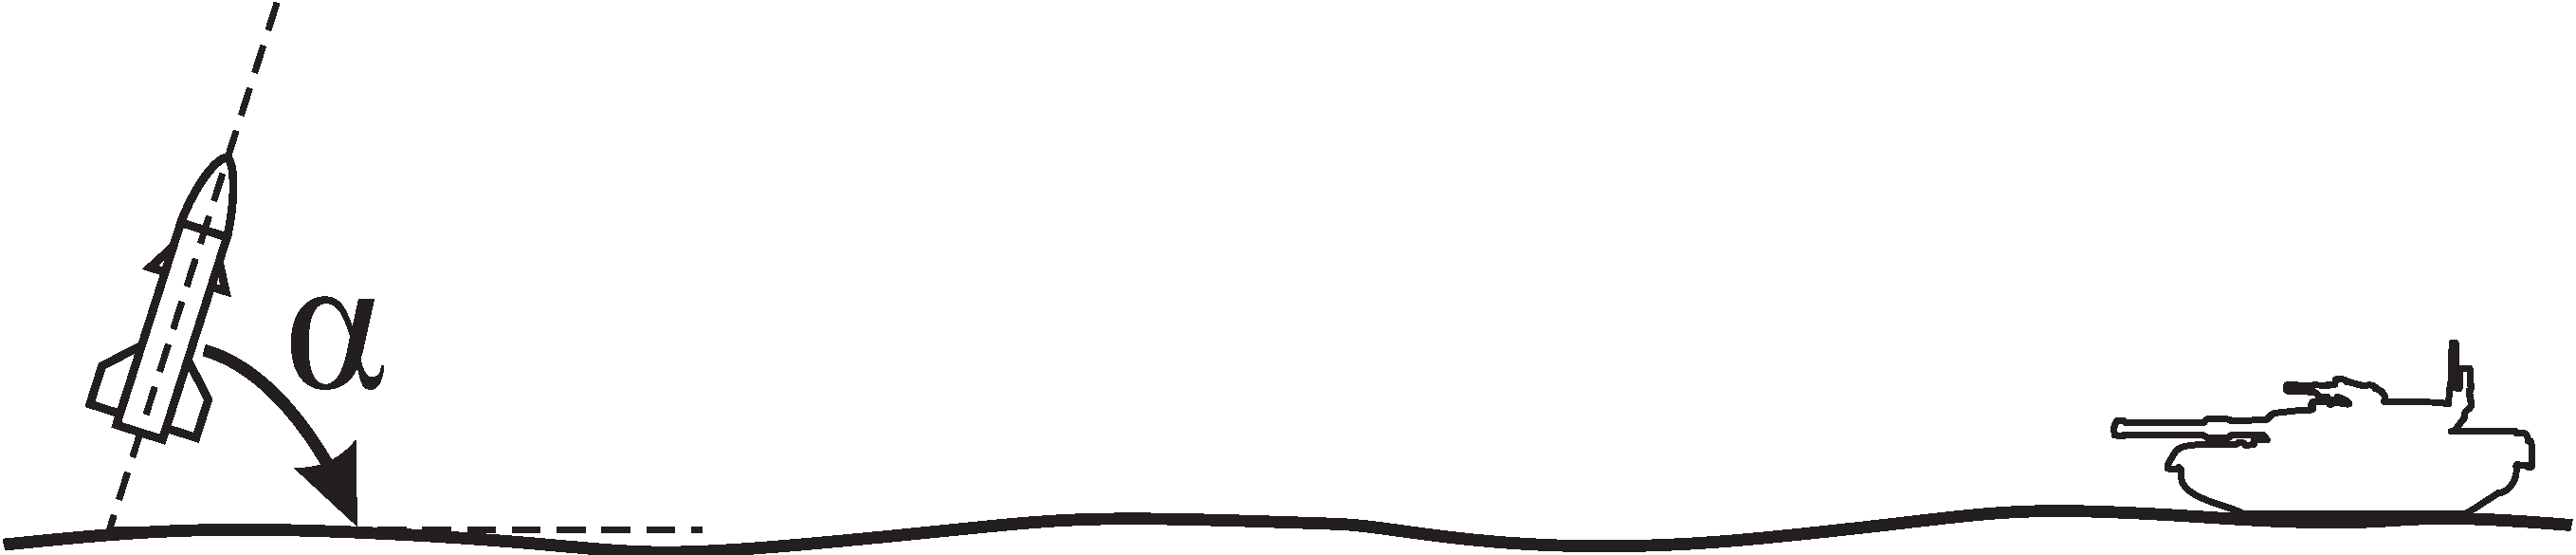
\includegraphics[width=0.475\textwidth]{rys05/alfa1} & 
  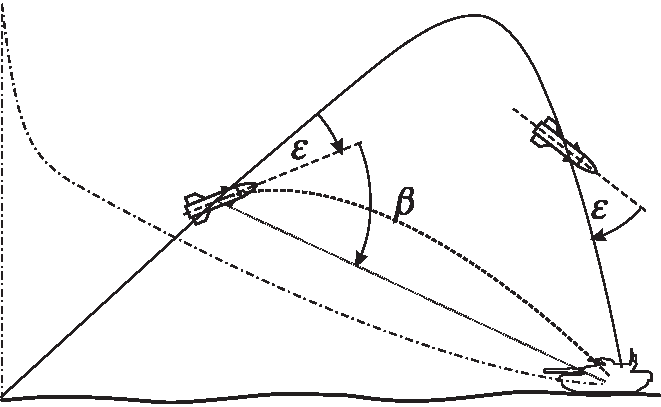
\includegraphics[width=0.475\textwidth]{rys05/beta1}
  \end{tabular}
 \caption{Wyznaczanie trajektorii lotu rakiety: 
 a) trzy podejścia, b) podejście praktyczne}
 \label{fig:alfabeta}
\end{figure}
\end{lstlisting}

\begin{figure}[ht]
	\centering
		
\includegraphics[width=0.3\linewidth]{rys05/kanji-giri}
	\caption{Dwa znaki kanji -- giri}
	\label{fig:kanji-giri}
\end{figure}

\begin{figure}[htb]
  \centering
	\begin{tabular}{@{}ll@{}}
	a) & b) \\
  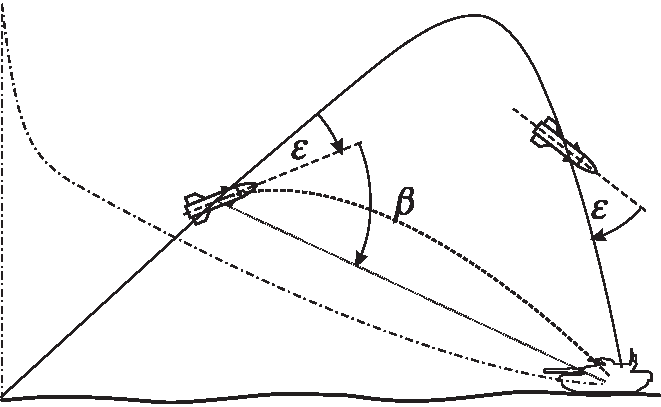
\includegraphics[width=0.475\textwidth]{rys05/beta1} & 
	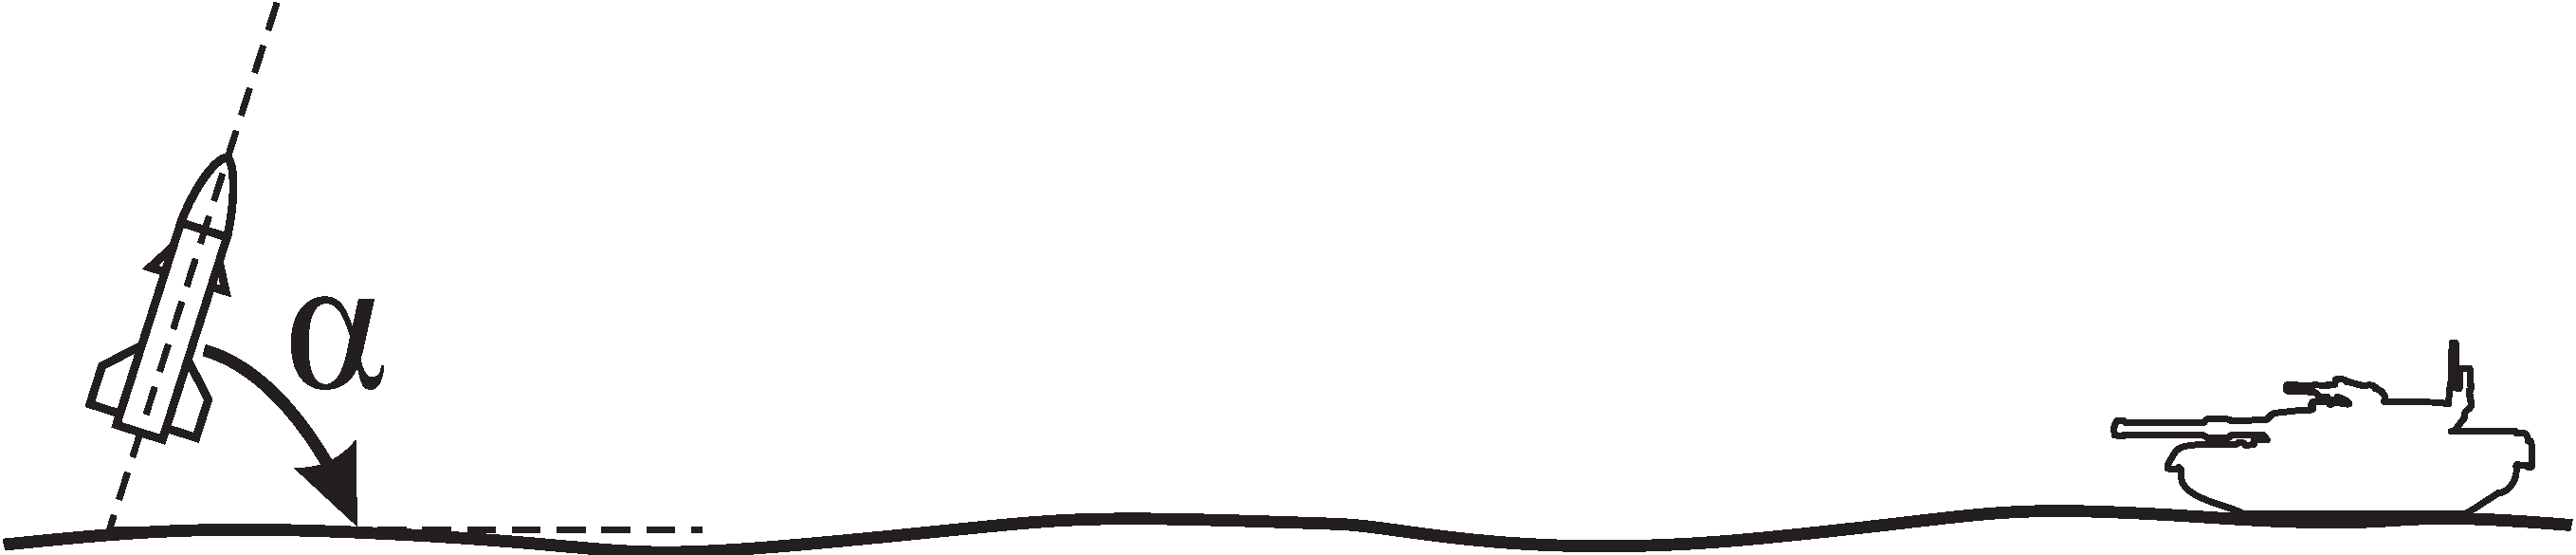
\includegraphics[width=0.475\textwidth]{rys05/alfa1}
	\end{tabular}
  \caption{Wyznaczanie trajektorii lotu rakiety: a) trzy podejścia, b) podejście praktyczne}
  \label{fig:alfabeta}
\end{figure}

Grafiki wektorowe powinny być dostarczone w plikach o formacie pdf. Rozmiar strony w~pliku pdf powinien być troszeczkę większy niż zamieszczona na nim grafika (proszę spojrzeć na przykłady grafik wykorzystanych w niniejszym szablonie). Chodzi o to, aby na rysunku nie pojawiała się niepotrzebna biała przestrzeń. Grafiki rastrowe (głównie zrzuty z ekranu bądź zdjęcia) powinny być dostarczane w plikach o formacie png z~kompresją bezstratną. Zastosowanie kompresji stratnej, jak jpg, wprowadza niepotrzebne artefakty. Podobnie jak w przypadku grafik wektorowych, grafiki rastrowe nie powinny mieć białych marginesów.

Na rysunkach nie powinno stosować się 100\% czarnego wypełnienia, bo robią się plamy przebijające się przez kartkę. Zamiast tego wypełnienie powinno być ok.\ 90\% czerni.

Czcionka na rysunkach nie może być większa od czcionki wiodącej tekstu (jedyny wyjątek to np.\ jakieś nagłówki).
Należy stosować czcionkę kroju Arial, Helvetica bądź tego samego kroju co czcionka dokumentu (\texttt{texgyre-termes}). 

Jeśli na jednym rysunku pojawić się ma kilka grafik, to zamiast stosować \texttt{subfigure} lub inne otoczenia należy wstawić grafiki w tabelę, opisać ją indeksami a) i b), a potem odnieść się do tego w podpisie (rys.~\ref{fig:alfabeta}).
Czasem pomaga w pozycjonowaniu rysunków użycie komendy:
\verb+\vtop{\vskip3ex\hbox{\includegraphics[width=0.475\textwidth]{nazwa}}}+

Na rysunkach nie wolno nadużywać kolorów oraz ozdobników (wiele narzędzi do tworzenia diagramów dostarcza grafikę z cieniowaniem, gradacją kolorów itp.\  co niekoniecznie przekłada się na czytelność rysunku).

Podczas rozbienia zrzutów z ekranu należy zadbać o to, by taki zrzut był czytelny po wydrukowaniu. Czyli aby pojawiające się literki były wystarczająco duże, a przestrzenie bez treści -- relatywnie małe.
Przystępując do robienia zrzutu trzeba odpowiednio wyskalować elementy na ekranie. Na przykład robiąc zrzut z przeglądarki FF najpierw należy wcisnąć CTR--0 (domyślne skalowanie), potem CTR--{}- (zmniejszenie skali o stopień). Potem dobrze jest zawęzić okno przeglądarki tak, by interesująca treść wypełniła je w całości. Jeśli na obserwowanej stronie jest zbyt dużo pustych obszarów, to należy je jakoś zawęzić (sterując wielkością okna przeglądarki lub aktywnymi elementami interfejsu użytkownika). Zrzut bowiem wcale nie musi być odzwierciedleniem 1:1 domyślnego układu obserwowanych elementów. Ważne jest, by na zrzucie z ekranu pokazać interesujący, opisywany fragment i żeby ten fragment był czytelny.
	
Czasem problemem jest tworzenie zrzutów z ekranu, gdy występują na nim dane wrażliwe. Istnieją dwa sposoby na radzenie sobie z tym problemem.
Pierwszy polega na zastąpieniu w~systemie danych danych rzeczywistych danymi testowymi -- wygenerowanymi tylko do celów prezentacji.
Zrzut robi się wtedy na bazie danych testowych.
Drugi polega na wykonaniu zrzutu z~ekranu, na którym pokazano dane rzeczywiste, i następnie zamianie tych danych już w pliku graficznym
za pomocą odpowiedniego edytora (np.~\texttt{gimp}). Czyli oryginalny zrzut z ekranu należy otworzyć w edytorze, a potem
nadpisać oryginalny tekst własnym tekstem. Konieczne jest wtedy dobranie odpowiednich czcionek aby nie było widać
wprowadzonych zmian. 
\begin{quotation}
Uwaga: takie manipulowanie zrzutami jest usprawiedliwione jedynie w przypadku konieczności ochrony danych wrażliwych czy też lepszego pokazania wybranych elementów. Nie może to prowadzić generowania fałszywych rezultatów!!!
\end{quotation}

\section{Wstawianie kodu źródłowego}
Kod źródłowy można wstawiać jako blok tekstu pisany czcionką maszynową. Używa się do tego otoczenie \verb?\lstlisting?. W atrybutach otoczenia można zdefiniować tekst podpisu wstawianego wraz z numerem nad blokiem, etykietę do tworzenia odwołań, sposób formatowania i~inne ustawienia. Zaleca się stosowanie w tym otoczeniu następujących parametrów:
\begin{lstlisting}[basicstyle=\footnotesize\ttfamily]
\begin{lstlisting}[label=list:req1,caption=Initial HTTP Request,
                   basicstyle=\footnotesize\ttfamily]
\end{lstlisting}
Szczególnie przydatne podczas wstawiania większej ilości kodu źródłowego jest zastosowanie parametru \verb+basicstyle=\footnotesize\ttfamily+. Dzięki niemu zmniejsza się czcionka, a~przez to na stronie można zmieścić dłuższe linijki kodu. Użycie tak zdefiniowanego parametru nie jest jednak sztywnym zaleceniem. Wielkość czcionki można dobierać do potrzeb. 
{\belowcaptionskip=-10pt
\begin{lstlisting}[label=list:req1,caption=Initial HTTP Request,
                   basicstyle=\footnotesize\ttfamily]
GET /script/Articles/Latest.aspx HTTP/1.1
Host: www.codeproject.com
Connection: keep-alive
Cache-Control: max-age=0
Accept: text/html,application/xhtml+xml,application/xml
User-Agent: Mozilla/5.0 ...
Accept-Encoding: gzip,deflate,sdch
Accept-Language: en-US...
Accept-Charset: windows-1251,utf-8...
\end{lstlisting}
}
Można też sformatować kod bez stosowania numerowanego podpisu (wtedy nie zamieszcza się \texttt{caption} na liście atrybutów).
\begin{lstlisting}[basicstyle=\footnotesize\ttfamily]
GET /script/Articles/Latest.aspx HTTP/1.1
Host: www.codeproject.com
Connection: keep-alive
Cache-Control: max-age=0
Accept: text/html,application/xhtml+xml,application/xml
User-Agent: Mozilla/5.0 ...
Accept-Encoding: gzip,deflate,sdch
Accept-Language: en-US...
Accept-Charset: windows-1251,utf-8...
\end{lstlisting}

Istnieje możliwość wstawiania kodu źródłowego w bieżącej linijce tekstu. Można to zrobić na kilka sposobów:
\begin{itemize} 
\item korzystając z polecenia \verb?\texttt? ustawiającego czcionkę maszynową, jak w przykładzie \texttt{tutaj} (efekt zastosowania komendy \verb?\texttt{tutaj}?). Problemem jednak mogą okazać się znaki podkreślenia i inne znaki kontrolne.
\item korzystają z otoczenia \verb?\verb? zapewniającego wypisanie kodu czcionką maszynową jak w~przykładzie \verb|tutaj| (efekt zastosowania komendy \verb?\verb|tutaj|?). Problemem jest to, że polecenie \verb?\verb? nie potrafi łamać dłuższego tekstu.
\item korzystając z polecenia \verb?\lstin? umożliwiającego wypisanie kodu czcionką ustawianą w~opcjach jak w przykładzie
\lstset{basicstyle=\ttfamily}\lstinline{tutaj} (efekt komendy \verb+\lstset{basicstyle=\ttfamily}\lstinline{tutaj}+) lub \lstinline[basicstyle=\ttfamily]=tutaj= (efekt komendy \verb+\lstinline[basicstyle=\ttfamily]=tutaj=+).
\end{itemize}

\section{Wykaz literatury oraz cytowania}
\label{sec:literatura}
Cytowania powinny być zamieszczane w tekście z użyciem komendy \verb+\cite{}+. Jej argumentem powinien być klucz cytowanej pozycji (lub lista kluczy  rozdzielonych przecinkiem bez spacji, jeśli takich pozycji w danym miejscu cytuje się więcej) jaki jest używany w bazie danych bibliograficznych (plik \texttt{dokumentacja.bib}). Po kompilacji \texttt{bibtex} i \texttt{pdflatex} w tekście pojawia się właściwy odsyłacz do pozycji w wykazie literatury (ujęty w kwadratowe nawiasy -- zgodnie z~tym, co definiuje styl \texttt{plabbrv.bst}), zaś w samym wykazie (rozdział Literatura) -- zacytowana pozycja. Przykładem cytowania jest: ,,dobrze to opisano w pracach~\cite{JS07,SQL2}'' (gdzie zastosowano komendę \verb?\cite{JS07,SQL2}?).

Co do zawartości rekordów bibliograficznych - style bibtexowe potrafią ,,skracać'' imiona (czyli wstawiać, jeśli taka wola, inicjały zamiast pełnych imion). Niemniej dobrze jest od razu przyjąć jakąś konwencję. Proponuje się, aby w rekordach od razu wstawiane były inicjały zamiast pełnych imion.

Niekiedy tytuły prac zawierają wyrazy z dużymi i małymi literami. Takie tytuły należy brać w podwójne nawiasy klamrowe, aby \texttt{bibtex} nie zamienił ich na postać, w której poza pierwszą literą pozostałe są małe.

Jeśli jakiś cytowany zasób pochodzi z Internetu, to jego rekord w pliku \texttt{bib} powinien wyglądać jak niżej.
\begin{lstlisting}[basicstyle=\footnotesize\ttfamily]
@INPROCEEDINGS{SQL2, 
  title={{A MySQL-based data archiver: preliminary results}}, 
  author={Bickley, M. and Slominski, Ch.},
  booktitle = {{Proceedings of ICALEPCS07}},
	month = oct,
	day = {15--19},
	year={2007}, 
  note={\url{http://www.osti.gov/scitech/servlets/purl/922267} 
	[dostęp dnia 20 czerwca 2015]}
}
\end{lstlisting}
A to inny przykład rekordu danych bibliograficznych:
\begin{lstlisting}[basicstyle=\footnotesize\ttfamily]
@TechReport{JS07,
	author = {Jędrzejczyk, J. and Śródka, B.},
	title  ={Segmentacja obrazów metodą drzew decyzyjnych},
	year = {2007},
	institution = {Politechnika Wrocławska, Wydział Elektroniki}
}
\end{lstlisting}

\section{Indeks rzeczowy}
\label{sec:indeks}
Generowanie indeksu \index{generowanie!-- indeksu} po trosze wygląda jak generowanie wykazu literatury \index{generowanie!-- wykazu literatury}-- wymaga kilku kroków. Podczas pierwszej kompilacji \texttt{pdflatex} generowany jest plik z rozszerzeniem \texttt{*.idx} (zawierający ,,surowy indeks''). Następnie, bazując na tym pliku, generowany jest plik z rozszerzeniem \texttt{*.ind} zawierający sformatowane dane. Ten krok wymaga uruchomienia odpowiedniego narzędzia oraz zastosowania plik z definicją stylu \texttt{Dyplom.ist}. W kroku ostatnim dokonuje się kolejnej kompilacji \texttt{pdflatex} (dzięki niej w wynikowym dokumencie pojawi się Indeks rzeczowy). Domyślnie Indeks rzeczowy zostanie sformatowany w~układzie dwukolumnowym.

Oczywiście aby to wszystko zadziałało w kodzie szablonu należy umieścić odpowiednie komendy definiujące elementy indeksu rzeczowego (\verb?\index?) oraz wstawiające sformatowany Indeks rzeczowy do dokumentu wynikowego (\verb?\printindex?). Więcej informacji o tworzeniu indeksu rzeczowego można znaleźć na stronie \url{https://en.wikibooks.org/wiki/LaTeX/Indexing}. Poniżej przedstawiono przykłady komend użytych w szablonie do zdefiniowania elementów indeksu rzeczowego:
\begin{itemize}
\item \verb?\index{linia komend}? -- pozycji główna.
\item \verb?\index{generowanie!-- indeksu}? -- podpozycja.
\end{itemize}

Generowanie pliku \texttt{*.ind} można inicjować na kilka sposobów:
\begin{itemize}
\item poprzez wydanie odpowiedniego polecenia bezpośrednio w linii komend \index{linia komend}
\begin{lstlisting}[basicstyle=\footnotesize\ttfamily]
makeindex Dyplom.idx -t Dyplom.ilg -o Dyplom.ind -s Dyplom.ist
\end{lstlisting}
\item poprzez odpalenie odpowiedniego narzędzia środowiska. Na przykład w \texttt{TeXnicCenter} definiuje się tzw. \texttt{output profiles}: 
\begin{lstlisting}[basicstyle=\footnotesize\ttfamily]
makeindex "%tm.idx" -t "%tm.ilg" -o "%tm.ind" -s "%tm.ist"
\end{lstlisting}
a samo generowanie pliku \texttt{*.ind} zapewni wybranie pozycji menu \texttt{Build/Makeindex}.
\item korzystając z odpowiednio sparametryzowanych pakietów i komend wewnątrz kompilowanego dokumentu (czyli od razu przy okazji jego kompilacji).
\begin{lstlisting}[basicstyle=\footnotesize\ttfamily]
\DisemulatePackage{imakeidx}
\usepackage[noautomatic]{imakeidx} 
% jeśli chcemy, by indeks by generowany automatycznie programem makeindex:
%\usepackage[makeindex]{imakeidx} 
% a tak ponoć można przekazać opcje do programu generującego indeks:
%\makeindex[options=-s podrecznik -L polish -M lang/polish/utf8] 
%\makeindex[options=-s podrecznik]
\makeindex
\end{lstlisting}

Niestety, \texttt{makeindex} jest narzędziem, które umieszcza część pozycji w grupie \texttt{Symbols}, a~nie w grupach związanych z literkami alfabetu (w związku z czym indeksowany element zaczynający się od polskiej literki trafia do grupy \texttt{Symbols}, jak np.~\verb?\index{Światło}?\index{Światło}. Jeśli chce się zamieszczać w indeksie symbole matematyczne, to dobrze jest to robić jak w następujacym przykładzie: \verb?\index{$asterisk@$\ast$}? \index{$asterisk@$\ast$} czy też \verb?\index{c@$\mathcal{C}$}?\index{c@$\mathcal{C}$}, tj.~dostarczając przy okazji klucz do sortowania.
Lepiej w tym względzie radzą sobie inne narzędzia, jak \texttt{texindy} lub \texttt{xindy} dostępne pod linuxem. Korzystając z nich uzyskuje się grupy polskich literek w indeksie rzeczowym (hasła zaczynające się od polskich literek już nie trafiają do grupy Symbols). Przykład polecenia wydanego z linii komend, w którym wykorzystano \texttt{texindy} zamieszczono poniżej (zakładamy kodowanie plików w UTF8, można dla niniejszego szablonu zmienić na cp1250):
\begin{lstlisting}[basicstyle=\footnotesize\ttfamily]
texindy -L polish -M lang/polish/utf8 Dyplom.idx
\end{lstlisting}

To polecenie wygeneruje \texttt{Dyplom.ind} o zawartości:
\begin{lstlisting}[basicstyle=\footnotesize\ttfamily]
\begin{theindex}
  \providecommand*\lettergroupDefault[1]{}
  \providecommand*\lettergroup[1]{%
      \par\textbf{#1}\par
      \nopagebreak
  }

  \lettergroup{G}
  \item generowanie
    \subitem -- indeksu, 27
    \subitem -- wykazu literatury, 27

  \indexspace

  \lettergroup{L}
  \item linia komend, 27

  \indexspace

  \lettergroup{Ś}
  \item \'Swiat\IeC {\l }o, 28

\end{theindex}
\end{lstlisting}


\end{itemize}


Aby mieć większą kontrolę automatyczne generowanie indeksu zostało w niniejszym szablonie wyłączone (indeks trzeba wygenerować samemu, wydając polecenie \texttt{makeindex} lub zalecane \texttt{texindy}).

\section{Inne uwagi}
Dobrym sposobem na kontrolę błędów występujących podczas kompilacji jest wstawiania linijki \verb?\end{document}? w wybranym miejscu dokumentu. Jest to szczególnie przydatne w przypadkach, gdy błędy te są trudne do zidentyfikowania (gdy wygenerowane przez kompilator numery linii z błędami nie są tymi, w których błędy występują). Wystarczy wtedy przestawić wspomnianą linijkę do kolejnych miejsc, aż znajduję to miejsce, gdzie występuje problem.

Aby osiągnąć apostrofy maszynowe (czyli takie złożone z samych kresek) należy użyć polecenia \verb?"{}jak tutaj{}"? (podwójny apostrof i podwójny apostrof z na wszelki wypadek umieszczonymi nawiasami klamrowymi, nawiasy są potrzebne z tej racji, iż podwójny apostrof przed niektórymi literkami zamienia je na literki z akcentami). W efekcie otrzymamy "{}jak tutaj{}". Jeśli natomiast apostrofy mają być drukarskie (czyli złożone z kropek i kresek), to należy użyć polecenia \verb?,,jak tutaj''? (dwa pojedyncze przecinki i dwa pojedyncze apostrofy). W efekcie otrzymamy ,,jak tutaj''. Można też użyć znaków apostrofów odpowiednio zakodowanych „jak tutaj”, tylko że czasem trudno pisze się takie apostrofy w środowiskach kompilacji projektów latexowych.


Oto sposoby ustawienia odstępów między liniami:
\begin{itemize}
\item używając komendy \verb+\linespread{...}+ (akceptowalne), przy czym atrybutem tej metody jest współczynnik zależny od wielkości
czcionki.  Dla czcionki wiodącej 12pt odstęp półtora linii osiągnie się komendą \verb+\linespread{1.241}+. Dla innych czcionek wiodących wartości tego parametru są jak w poniższym zestawieniu.
\begin{lstlisting}[basicstyle=\footnotesize\ttfamily]
10pt 1.25 dla \onehalfspacing 
     1.667 for \doublespacing, 
		 ponieważ ,,basic ratio'' = 1.2 
		(\normalfont posiada \baselineskip rozmiaru 12pt)
11pt 1.213 dla \onehalfspacing oraz 1.618 dla \doublespacing, 
     ponieważ ,,basic ratio'' = 1.236 
		(\normalfont posiada \baselineskip rozmiaru 13.6pt)
12pt 1.241 dla \onehalfspacing oraz 1.655 dla \doublespacing, 
     ponieważsince ''basic ratio'' is 1.208 
		(\normalfont has a \baselineskip of 14.5pt)
\end{lstlisting}
Kłopot w tym, że raz ustawiony odstęp będzie obowiązywał do wszystkich czcionek (nie działa tu żadem mechanizm zmiany współczynnika w zależności od wielkości czcionki akapitu).

\item używając pakietu \texttt{setspace} (niezalecane). Ponieważ klasa \texttt{memoir} emuluje pakiet \texttt{setspace}, w preambule dokumentu należałoby umieścić:
\begin{lstlisting}[basicstyle=\footnotesize\ttfamily]
\DisemulatePackage{setspace}
\usepackage{setspace}
\end{lstlisting}
a potem można już sterować odstęp komendami:
\begin{lstlisting}[basicstyle=\footnotesize\ttfamily]
\singlespacing
\onehalfspacing
\doubelspacing
\end{lstlisting}
Ten sposób pozwala na korzystanie z mechanizmu automatycznej zmiany odległości linii w~zależności od wielkości czcionki danego akapitu.
\item korzystając bezpośrednio z komend dostarczonych w klasie \texttt{memoir} (zalecane):
\begin{lstlisting}[basicstyle=\footnotesize\ttfamily]
\SingleSpacing
\OnehalfSpacing
\DoubleSpacing
\end{lstlisting}
Ten sposób również pozwala na korzystanie z mechanizmu automatycznej zmiany odległości linii w zależności od wielkości czcionki danego akapitu.
\end{itemize}

Na koniec jeszcze uwaga o rozmiarze pliku wynikowego. Otóż \texttt{pdflatex} generuje pliki \texttt{pdf}, które zazwyczaj mogłyby być nieco lepiej
skompresowane. Do lepszego skompresowania tych plików można użyć programu \texttt{ghostscript}. Wystarczy w tym celu wydać komendę (pod windowsami):
\begin{lstlisting}[basicstyle=\footnotesize\ttfamily]
gswin64 -sDEVICE=pdfwrite -dCompatibilityLevel=1.4 -dNOPAUSE -dQUIET -dBATCH 
-sOutputFile=Dyplom-compressed.pdf Dyplom.pdf
\end{lstlisting}

% \chapter{Podsumowanie}
\label{chap:podsumowanie}
Lorem ipsum dolor sit amet eleifend et, congue arcu. Morbi tellus sit amet, massa. Vivamus est id risus. Sed sit amet, libero. Aenean ac ipsum. Mauris vel lectus. 

\section{Sekcja poziomu 1}% 
Lorem ipsum dolor sit amet eleifend et, congue arcu. Morbi tellus sit amet, massa. Vivamus est id risus. Sed sit amet, libero. Aenean ac ipsum. Mauris vel lectus. 

Nam id nulla a adipiscing tortor, dictum ut, lobortis urna. Donec non dui. Cras tempus orci ipsum, molestie quis, lacinia varius nunc, rhoncus purus, consectetuer congue risus. 

\subsection{Sekcja poziomu 2}
Lorem ipsum dolor sit amet eleifend et, congue arcu. Morbi tellus sit amet, massa. Vivamus est id risus. Sed sit amet, libero. Aenean ac ipsum. Mauris vel lectus. 
\subsubsection{Sekcja poziomu 3}
Lorem ipsum dolor sit amet eleifend et, congue arcu. Morbi tellus sit amet, massa. Vivamus est id risus. Sed sit amet, libero. Aenean ac ipsum. Mauris vel lectus. 
\paragraph{Paragraf 4}
Lorem ipsum dolor sit amet eleifend et, congue arcu. Morbi tellus sit amet, massa. Vivamus est id risus. Sed sit amet, libero. Aenean ac ipsum. Mauris vel lectus. 
\section{Sekcja poziomu 1}% 
Lorem ipsum dolor sit amet eleifend et, congue arcu. Morbi tellus sit amet, massa. Vivamus est id risus. Sed sit amet, libero. Aenean ac ipsum. Mauris vel lectus. 
\cite{BPMN}
%\show\chapter
%\show\section
%\show\subsection

%\showthe\secindent
%\showthe\beforesecskip
%\showthe\aftersecskip
%\showthe\secheadstyle
%\showthe\subsecindent
%\showthe\beforesubsecskip
%\showthe\aftersubsecskip
%\showthe\subseccheadstyle
%\showthe\parskip


\newpage
\mbox{}\pdfbookmark[0]{Spis rysunków}{spisRysunkow.1}
%\addcontentsline{toc}{chapter}{Spis rysunków}
\listoffigures*

% \newpage
% \mbox{}\pdfbookmark[0]{Spis tabel}{spisTabel.1}
% %\addcontentsline{toc}{chapter}{Spis tabel}
% \listoftables*

%\bibliographystyle{plalpha}
\bibliographystyle{plabbrv}

%UWAGA: bibliotekę referencji należy przygotować samemu. Dobrym do tego narzędziem jest JabRef.
%       Nazwę przygotowanej biblioteki wpisuje się poniżej bez rozszerzenia 
%       (w tym przypadku jest to "dokumentacja.bib")
\bibliography{dokumentacja}
\appendix
\chapter{Opis załączonej płyty CD/DVD}
Tutaj jest miejsce na zamieszczenie opisu zawartości załączonej płyty.
Należy wymienić, co zawiera.


\chapterstyle{noNumbered}
\phantomsection % sets an anchor
\addcontentsline{toc}{chapter}{Indeks rzeczowy}
\printindex

\end{document}
